\documentclass[11pt,letterpaper]{article}
\usepackage{nsfproposal}
\usepackage{bm}
\usepackage{amsthm}
\usepackage{color,xcolor,colortbl} 
\usepackage{hyperref} 
\usepackage{graphicx} 
\usepackage{vmargin} 
\usepackage{enumitem, soul}
\usepackage{amsmath,amssymb,xspace, comment}
\usepackage{tikz}
\usepackage{multirow}
\usepackage{graphicx}
\usepackage{booktabs,wrapfig}
\usepackage{makecell}
\usepackage{array}
\usepackage{longtable}
\usepackage{tabularray}
\usepackage{tcolorbox}
\usepackage{mfirstuc}
\usepackage{makecell}
\usepackage{algorithm}
\usepackage{algpseudocode}
\usepackage{rotating}
\usepackage{tabularray}
\usepackage{wasysym}

\MFUnocap{are}
\MFUnocap{or}
\MFUnocap{etc}
\MFUnocap{and}
\MFUnocap{with}
\MFUnocap{of}
\MFUnocap{a}


\newtcolorbox{goalsbox}[2][]
{
  colframe = #2!25,
  colback  = #2!10,
  coltitle = #2!20!black,  
  #1,
}

\setpapersize{USletter}
\setmarginsrb{1in}{1in}{1in}{1in}{0pt}{0mm}{0pt}{0mm}


\renewcommand*{\thefootnote}{\fnsymbol{footnote}}
\newcommand{\pseudodot}{{\lower 2.4pt\hbox{$\cdot$}}}
\renewcommand{\title}[1]{\begin{center}\LARGE\bfseries{#1}\end{center}}
\setul{0.8pt}{}
\sodef\an{}{-.02em}{0.2em plus0.2em}{0.5em plus.1em minus.1em}

\newcommand*\cib[1]{\tikz[baseline=(char.base)]{
                \node[shape=circle,fill=black,text=white,draw,inner sep=0.3pt] (char) {#1};}}

\hypersetup{colorlinks=true,citecolor=blue,linkcolor=blue,urlcolor=blue}
\newcommand{\etal}{{\em et al.}\xspace}
\newcommand{\eg}{{\em e.g.,}\xspace}
\newcommand{\ie}{{\em i.e.,}\xspace}
\newcommand{\etc}{{\em etc.}\xspace}
% \renewcommand{\sectionautorefname}{{\S\hspace{-0.5ex}}}
% \renewcommand{\subsectionautorefname}{{\S\hspace{-0.5ex}}}
% \renewcommand{\subsectionautorefname}{Table}
\newcommand{\algorithmautorefname}{Algorithm}
\renewcommand{\tableautorefname}{Table}
\renewcommand{\itemautorefname}{Table}
\renewcommand{\equationautorefname}{Eq.\hspace{-0.5ex}}
\newcommand{\argmin}{\mathop{\mathrm{arg\,min}}}
\newcommand{\argmax}{\mathop{\mathrm{arg\,max}}}

\newcommand{\xo}{\raisebox{0.4ex}{\textbf{$\chi$}}\xspace}
\newcommand{\xod}{{{\xo}-embodied}\xspace}
\newcommand{\xot}{{{\xo}-embodiment}\xspace}
\newcommand{\ours}{{\small$\textsf{{X}-RSecure}$}\xspace}
\newcommand{\BfPara}[1]{{\noindent\bfseries\an{#1}.}\xspace}
\newcommand{\BfParaUL}[1]{{\noindent\ul{\textbf{#1}.}}\xspace}
\newcommand{\dd}{\Circle}
\newcommand{\vv}{\CIRCLE}
\newcommand{\bb}{\RIGHTcircle}
\newcommand{\ee}{$\cdot$}
\newcommand{\BfParaC}[1]{{\vspace{1ex}\noindent\bfseries{\capitalisewords{#1}.}\xspace}}

\newcommand{\todo}[1]{\textcolor{blue}{[$\rightarrow$#1]}}
\newcommand{\mo}[1]{\textcolor{red!85!black}{#1}}
\usepackage{txfonts}
\renewcommand{\rmdefault}{txr}
% \usepackage{algpseudocode}
% \usepackage[linesnumbered]{algorithm2e}

\usepackage{tcolorbox}
\tcbuselibrary{theorems}


% 


\newtcbtheorem[]{observation}{\textbf{}}%
{colframe=white!95!black,fonttitle=\bfseries,coltitle=black, boxsep = 2pt, left = 0pt, right = 0pt, top = 1pt, bottom = 2pt, boxrule = 0pt, bottomrule = 0pt, toprule = 0pt}{th}{}


\newtheoremstyle{styledef}%
{\topsep}% Space above
{\topsep}% Space below 
{}% Body font
{3pt}% Indent amount
{\bfseries}% Theorem head font
{.}% Punctuation after theorem head
{3pt}% Space after theorem head
{}% Theorem head spec (can be left empty, meaning ‘normal’)
\theoremstyle{styledef}

%\newtheorem{observation}{Observation}

\newcommand{\observationdef}[2][0.97\textwidth]{
  \vspace{2ex}\par\noindent\tikzstyle{mybox} = [fill=gray!10,
   thick,rectangle,inner sep=6pt,path picture={\fill [white!40!black] ([xshift=-8.1cm]path picture bounding box.north) rectangle (path picture bounding box.south west);}]
  \begin{tikzpicture}
  \centering
   \node [mybox] (box){%
    \begin{minipage}{#1}{ #2}\end{minipage}
   };
  \end{tikzpicture}
}

\setlength{\baselineskip}{12.6pt} % in text mode
\setlength{\normalbaselineskip}{12.6pt} % in math mode

\usetikzlibrary{positioning}


% Make all figure and table captions small
\usepackage{caption}
\captionsetup[figure]{font=small}
\captionsetup[table]{font=small}





\begin{document}
\pagestyle{empty} 


\setlength{\baselineskip}{12.6pt} % in text mode
\setlength{\normalbaselineskip}{12.6pt} % in math mode
\title{\Large
SaTC 2.0: RES: Toward Secure and Robust Generalist Robotic  Models} 
\begin{center}
   {\bfseries\filcenter} ~\vspace{2ex}
   {\Large\bfseries\filcenter
Project Description
\\\rule{\textwidth}{0.4pt}}
%Mohammed Abuhamad, Loyola University Chicago} 
\end{center}


\section{Overview}

Generalist ``foundation'' robot models are the next revolutionary step toward the widespread adoption of intelligent and robust robotic systems. 
Inspired by the tremendous advancements in large language, vision, and vision-language models, the development of robotic foundation models is just beginning. 
However, ensuring their security, safety, and trustworthiness remains a significant challenge. Building on these models, system designers need comprehensive frameworks, advanced security measures, and specialized methods to build secure, safe, and reliable models for downstream tasks. This proposal aims to address these critical needs, improving the security and trustworthiness of foundation robot models for real-world deployment. We define trust as the assurance that a robotic foundation model produces safe, intended physical actions under both benign and adversarial multimodal inputs.

Millions of industrial robots (\eg in logistics and manufacturing) and service robots (\eg in medicine, home, transportation, defense, and military) are poised to become smarter and more reliable with advances in these foundation models. The previous barrier to the emergence of large robotic foundation models, namely, the need for large-scale ``Internet-wide'' datasets as seen in large language models (LLMs) and vision-language models (VLMs), has diminished. Recent efforts employ large-scale \xot robotic datasets and new training methods, making this challenge less critical and paving the way for significant advancements.
Current efforts to build robotic foundation models, \eg Large Language-Vision-Action (VLA) models, focus on integrating various pre-trained models (\eg vision models, LLMs, and VLMs) for multiple modalities (\eg visual and textual instructions) used by robots. 
The transfer learning capabilities of these components enable robotic systems to reason, interact, and learn new tasks in diverse environments. However, this raises concerns about potential security and safety issues that might be inherited from these models, along with the adversarial threats they may face.

\vspace{-2ex}
%This proposal seeks to fill the gap in hardware platforms, runtime systems, and tools for practical, dynamic, and capable applications on intermittently powered embedded systems.
\observationdef{
\begin{observation*}{}{}
\vspace{-1ex}\textbf{This proposal seeks to address the security and trustworthiness challenges in developing foundation models for robotics, ensuring robust frameworks and defense mechanisms for integrating various pre-trained models, and securing against inherited vulnerabilities and adversarial threats.}
\vspace{-1ex}
\end{observation*}
}
\vspace{-3ex}

Neural network-based models are susceptible to adversarial manipulations, where small, undetected perturbations to the input can drastically alter the output (\eg targeting a specific output or a random incorrect output). Unlike the mature research on studying vulnerabilities in vision and LLMs, which have been the theme of AI security research for many researchers, including the PI, robotics is just beginning to tackle the complexities of securing large models. The real-time interaction of robots with dynamic environments introduces numerous attack vectors that could induce harmful behaviors, leading to safety hazards and operational failures. 
Moreover, the integration of multiple modalities in robotics creates a complex and largely unexplored attack surface, where subtle input data manipulations can significantly degrade performance.
Investigating these vulnerabilities is imperative for developing robust defense mechanisms tailored to the specific requirements of robotic systems. 
The lack of comprehensive security studies and evaluation benchmarks in this field highlights the need for dedicated research to identify and mitigate the risks associated with the use of these models. Ensuring the safe deployment of robotic technologies across various applications requires a focused effort to understand and address these security challenges, paving the way for secure and reliable robotic operations in dynamic and unseen environments.

This project builds and examines diverse models using real-world \xot datasets for various robots with different embodiments and builds security frameworks and benchmarks to address these urgent shortfalls in emerging robotic foundation models. This work enables the development and adoption of secure and trustworthy robotic models in real-world applications.
The project promotes public acceptance and trust in robotics and impacts the community by developing comprehensive curriculum modules, organizing seminars, and promoting active research participation for high school and undergraduate students.
% Educational initiatives aim to foster interest in secure robotics and responsible AI, and provide practical, hands-on learning opportunities.







% \newpage
\subsection{Vision, Goals, and Technical Approach}
%This proposal advocates for a future
~{%\vspace{-1ex}}
\begin{wrapfigure}{r}{0.25\textwidth}%\vspace{-2ex}
  \centering
  \begin{minipage}{0.25\textwidth}
    \centering
  \vspace{-9ex}
  \includegraphics[width=0.9\textwidth]{figures/rtx_resultss.pdf}\vspace{-2ex}
  \caption{{\scriptsize Results of end-to-end {\xo}-embodied robot learning.}}\vspace{3ex}
  \label{fig:rt-x_result}
  \end{minipage}
  \hfill \vspace{-3.5ex}
\begin{minipage}{0.25\textwidth}
  \centering
  {\scalebox{0.9}{%
  \begin{minipage}{0.15\textwidth}
    \centering
      \rotatebox{90}{{(A)}}~\hfill
  \end{minipage}~\hspace{-5.5ex}
  \begin{minipage}{1.3\textwidth}
    \begin{minipage}{0.99\textwidth}
    \centering
    \includegraphics[width=0.395\textwidth]{figures/examples/dolphin.pdf}%
    \includegraphics[width=0.385\textwidth]{figures/examples/jackel.pdf}%
    \vspace{-1ex}
  \end{minipage}
  \begin{minipage}{0.99\textwidth}
    \centering
    \includegraphics[width=0.390\textwidth, trim={0 10pt 0 0}, clip]{figures/examples/go2.pdf}%
    \includegraphics[width=0.390\textwidth,trim={0 10pt 15pt 20pt}, clip]{figures/examples/go22.pdf}%
  \end{minipage}
  \end{minipage}}
   %
  \scalebox{0.9}{
  \hspace{-0.8ex}\begin{minipage}{0.15\textwidth}
    \centering
      \rotatebox{90}{(B)}~\hfill
  \end{minipage}~\hspace{-5.5ex}
  \begin{minipage}{1.3\textwidth}
    \centering
    \includegraphics[width=0.39\textwidth]{figures/examples/a_quad_real.pdf}%
    \includegraphics[width=0.39\textwidth]{figures/examples/a_quad_sim.pdf}%
  \end{minipage}}%
  }
  \vspace{-2ex}

  
  \caption{\scriptsize (A) Jailbreak attacks \cite{robey2024jailbreaking} that causing harmful robotic actions, including collision with humans, bomb detonation, and weapon retrieval. 
    (B) Subtle perturbations (bounded by just $3^{\circ}$) \cite{shi2024rethinking} causing  failure in quadruped locomotion.}
  \vspace{3ex}
  \label{fig:examples}
\end{minipage}
\end{wrapfigure}
\vspace{-5ex}

%\BfPara{Security in Robotic Learning Towards Generalist {\xo}-embodied Robots}
\noindent This proposal advocates for a future with secure, trustworthy, and safe large generalist robotic models.
Creating robot manipulators capable of performing successfully in various scenarios has been a persistent objective in robotics research \cite{kaelbling2020foundation,9,rt-1,rt-2,zhang2024vla}. 
Recent studies have shown that generalization in robotic manipulation can be achieved using large and diverse datasets~\cite{pinto2016supersizing,kaelbling2020foundation,levine2018learning,xu2025vla,arai2025covla}. Robots can learn
new objects~\cite{pinto2016supersizing,levine2018learning,finn2017deep,young2021visual,9},  tasks~\cite{james2018task,dasari2021transformers,jang2022bc,9},  instructions and goals~\cite{nair2022learning,jang2022bc,jiang2023vima,mees2022matters}, and unseen environments~\cite{hansen2020self,cui2022play,9}. 
For example, $\text{RT-2-}_\text{PaLM-E-12B}$~\cite{rt-2} achieved {93}\% overall success in seen tasks, and {62}\% average success on unseen objects, backgrounds, and environments. 
Building a single end-to-end model that generalizes to unforeseen conditions across all these dimensions is becoming a reality~\cite{rt-1,rt-2,9,wen2025tinyvla,xu2025vla}, aligning with developments in vision and language models where large general models are pre-trained on large-scale datasets with task-agnostic open-ended training. 
Moreover, training robots with \xot datasets can help improve their performance~\cite{9}, as shown in \autoref{fig:rt-x_result}.
Like other neural networks, end-to-end robotic models can be vulnerable to adversarial manipulations despite tolerating input noise.
% Recent studies \cite{robey2024jailbreaking} shows successful jailbreak attacks on LLM-controlled robots (\autoref{fig:examples}-A) and
%  ~\cite{shi2024rethinking} reveals adversarial vulnerabilities in quadrupedal locomotion controllers, including the DARPA Subterranean Challenge-winning policy~\cite{miki2022scirob,rslsubt2022} (\autoref{fig:examples}-B).
Recent studies revealed alarming security vulnerabilities in robotic systems: \cite{robey2024jailbreaking} successfully executed jailbreak attacks on LLM-controlled robots (\autoref{fig:examples}-A), while \cite{shi2024rethinking} exposed critical adversarial vulnerabilities in quadrupedal locomotion controllers, including the DARPA Subterranean Challenge-winning policy \cite{miki2022scirob,rslsubt2022} (\autoref{fig:examples}-B).
\emph{We must investigate the uncharted threat landscape of robotic foundation models, including the vision, language, and/or vision-language backbone models used in end-to-end learning.}

Emerging industry efforts, \eg Google's RT-1 and RT-2, Nvidia's Eureka, OpenAI's RFM-1, Meta's V-JEPA 2, and Tesla's Optimus show that using large high-capacity robotic models to transfer knowledge from large and diverse datasets can achieve high performance on robot-specific tasks even with smaller datasets. 
This trend is also evident in academia and national laboratories around the globe (\eg VLA~\cite{kim2024openvla}, Octo~\cite{team2024octo}, Orion~\cite{fu2025orion}, Pi-0~\cite{black2024pi_0}, DexVLA~\cite{wen2025dexvla}, \etc), and is expected to continue. 
The open \xot \cite{9} project published a large \xot robotic dataset and shows that robots achieve better generalization when trained on such datasets.
The democratization of these models and resources promises continuous growth in generalist robots.
Despite this progress, the security and trustworthiness of generalist robots remain underexplored. Recent works have begun exposing isolated vulnerabilities, including jailbreaking of LLM-controlled robots~\cite{robey2024jailbreaking}, adversarial attacks on quadrupedal locomotion~\cite{shi2024rethinking}, and emerging backdoor and adversarial attacks on vision-language-action models~\cite{badvla,advvla}. These efforts target isolated components or single models rather than the end-to-end robotic learning pipeline.
This proposal presents the first comprehensive framework unifying threat modeling, cross-modal analysis, and defenses and benchmarks, addressing this gap through three conceptual and practical ideas: 


\BfPara{{\cib{1}} Comprehensive Framework against Vast Threat Landscape}
Considering the large threat vector from data/task complexity,
we need to implement a robotic security framework that combines systematic threat modeling, vulnerability assessment, and cross-disciplinary attack taxonomies.
This framework will help understand the adversarial strategies that can be employed against robots (\ie with different embodiments/environments/tasks). 
Bridging the gap across fields, \ie AI, cybersecurity, and robotics, will help the holistic understanding of the threat landscape and guide future research to identify threats and defenses.

\BfPara{{\cib{2}} Investigation of Modality-Specific Vulnerabilities in Multimodal Robotics} Incorporating LLMs, VLMs, and VLAs into training robotic policies dictates investigating the unique vulnerabilities of each modality, such as textual instruction, visual guidance, and actions, and how these inputs impact robot actions. 
Although many studies focus on adversarial attacks against single modalities, little work has been done on multimodal adversarial techniques. {We must identify areas of strengths and potential weaknesses in end-to-end multimodal robotic training pipeline, and advise measures to improve the security and safety of the system.}

\BfPara{{\cib{3}} Benchmarks for Robustness and Trustworthiness}
    Research must prioritize the development of evaluation frameworks that rigorously test the robustness and trustworthiness of robotic systems, ensuring that they can withstand adversarial conditions and maintain high ethical/safety standards. This is essential for building reliable generalist robots that can be trusted to operate autonomously in diverse and dynamic environments.
    






\begin{figure*}[ht]
  \centering
  \vspace{-1.5ex}
  \includegraphics[width=\textwidth]{figures/pipeline_6.pdf}\vspace{-2ex}
  \caption{\textbf{Toward Secure, Trustworthy, End-to-End Robotic Models.} Gaps, Challenges, and Proposed Work.}
  \vspace{-4ex}
  \label{fig:pipeline}
\end{figure*}







% The work in this proposal revolves around the development of a secure and trustworthy end-to-end robotic ecosystem.
Building a secure and trustworthy end-to-end robotic learning paradigm is an interconnected approach that redefines core concepts in the context of robotics. An overview of our approach and vision, including tasks and key ideas, is shown in \autoref{fig:pipeline}. 
We consider various robot embodiments (\eg single robot arms, bi-manual robots, and quadrupeds) and a combination of 15 datasets including the Open {\xo}-Embodiment (OXE)~\cite{9} repository, which contains 60 robotic datasets.
Focusing on \textbf{multimodal robots}, we use data for {six robots, six embodiments, and 15 datasets} across experiments (see \autoref{tab:multi_dataset})
% Freiburg Franka Play~\cite{rosete2022tacorl,mees23hulc2},
% Maniskill~\cite{gu2023maniskill2},
% Stanford Robocook~\cite{shi2023robocook},
% CMU Franka Pick-Insert Data~\cite{saxena2023multiresolution},
% RoboVQA~\cite{9},
% DROID~\cite{khazatsky2024droid},
% ConqHose~\cite{ConqHoseManipData},
% DobbE~\cite{shafiullah2023dobbe},
% FMB~\cite{luo2024fmb},
% IO-AI Office PicknPlace~\cite{9},
% RoboSet~\cite{bharadhwaj2023roboagent},
% VIMA~\cite{jiang2023vima},
% SPOC~\cite{spoc2023}
to build end-to-end robot agents. %, \eg %RT-1~\cite{rt-1}, RT-2~\cite{rt-2}, RT-X~\cite{9}, ACT~\cite{zhao2023learningFB}, and OpenVLA~\cite{kim2024openvla}. 
We leverage other datasets/benchmarks to train/fine-tune backbone VLMs, VLAs, visual encoders, and LLMs.
When we push on all fronts to explore the space to its fullest extent, we may uncover new research challenges and better equip the research community to tackle them. Each research task presents numerous interesting problems to explore and overcome. 
%The work is wide-ranging and involves building real systems and tools, including software and hardware artifacts, and evaluating them with real data, deployments, and robots. 
Foundation models for end-to-end robotic agents will be adopted and democratized in various platforms and industries in the near future, and our vision can be realized by conducting the following research tasks.




%The BFree Ecosystem for Battery-free, Energy Harvesting, Failure Resilient Embedded Computing: a holistic approach to prototyping, designing, testing, programming, and deploying battery-free smart devices.







\BfPara{T1: Vulnerability Analysis in Foundation Generalist Robots} 
To address the large threat vector from data and task complexity, we will conduct comprehensive threat assessments and vulnerability analysis. The approach involves collecting and categorizing diverse data sources and tasks that robots encounter. We will develop detailed taxonomies of potential attacks, focusing on \textit{evasion}, \textit{poisoning}, and \textit{privacy} attacks for predictive models, as well as additional \textit{abuse} (\eg jailbreak) attacks for generative models. Implementation includes compiling a dataset of known threats, performing simulated attack scenarios in controlled environments, and using adversarial machine learning to analyze vulnerabilities. Detailed documentation of each identified vulnerability and its impact on various robotic applications will be maintained. Collaborative workshops with experts from AI, cybersecurity, and robotics will ensure a multidisciplinary perspective, and periodic reviews will be conducted to update the taxonomy with emerging threats.
%TODO: add more deliverables.


\BfPara{T2: Modality-inherited Vulnerabilities and Impact on Multimodal Robots} 
Incorporating large VLMs, VLAs, and LLMs into robotic training policies requires investigating the vulnerabilities of each modality and the underlying backbone model. 
This task will focus on textual instruction, visual guidance, and actions, studying their unique impacts on robot behavior. 
The approach involves designing and building adversarial attacks across different modalities and monitoring their effects on robotic actions to uncover/identify vulnerabilities. 
We will propose defense mechanisms and evaluate their effects against attacks.
%TODO: add more deliverables.
%The task will culminate in a comprehensive report detailing the vulnerabilities, their impacts, and proposed mitigation strategies, along with open-source tools for the community to replicate and build upon our findings.



\BfPara{T3: Benchmarks Toward Safe and Trustworthy Robotic Models} 
% This task involves creating a comprehensive assessment benchmarks of \textit{interpretability} and \textit{safety} in generalist robots. The approach includes designing benchmark tests that simulate a variety of adversarial conditions and ethical dilemmas. 
% We will use both real-world scenarios and controlled environments to conduct experiments and design new methods to improve robustness, interpretability, safety, and fairness.
% Additionally, we will employ tools to ensure that robots do not inherit vulnerabilities from large-backbone models. 
As robotic systems are increasingly adopted and democratized, ensuring their safety and interpretability is crucial. 
Extending beyond traditional physical safety standards, we need to examine models' output safety under various conditions (both normal and adversarial). 
This task aims to establish comprehensive benchmarks and open-source tools for evaluating and enhancing \emph{safety} and \emph{interpretability} in robotic foundation models. 
%It addresses the critical need for trustworthy robotic systems that operate reliably in human environments,. %The goal is to establish standardized benchmarks and open-source tools that enable systematic evaluation of robotic systems under diverse conditions.






\subsection{Intellectual Merit}
The proposed work initiates, prioritizes, and provides a comprehensive approach to enhance the security and robustness of large foundation models in robotics through three main pioneering contributions: \cib{1} developing the first comprehensive taxonomy and framework of threat vectors specific to multimodal robotic systems across diverse embodiments and tasks, \cib{2} establishing novel methodologies to analyze cross-modal attack propagation that reveal previously unexplored vulnerabilities in vision-language-action integration, and \cib{3} creating standardized benchmarks and evaluation frameworks for robotic security, safety, and interpretability that bridge the critical gap between AI, cybersecurity, and robotics.
Concretely, we propose to develop two VLA-specific attack primitives exploiting mechanisms absent in VLMs: Action-Bin Boundary Perturbation (ABBP), a gradient-based attack driving predicted action tokens across the boundaries of the 256-bin action quantization under a kinematically-consistent constraint across degrees of freedom, and the Temporal Trajectory Drift Attack (TTDA), exploiting the temporal action-chunk structure of multi-step policies. We further propose two robotics-specific defenses, a Temporal Action Consistency Detector (TACD) operating at the trajectory level and Action-Grounded Adversarial Fine-Tuning (AGAT) using kinematically-constrained perturbations. We will release these components through VLA-SecBench, an open benchmark providing a cross-model transferability matrix and a spatial-action interpretability tool. We frame these contributions as proposed research to be validated rather than completed results.
The research spans two complementary tracks led by a two-investigator team, a PI with expertise in AI/ML security and adversarial machine learning and a Co-PI [Co-PI: TBD] contributing robot-learning and real-robot experimentation expertise, enabling parallel progress on the security and robotics tracks.
The project will produce practical outcomes, such as security-enhanced versions of foundational robotics models along with open-source attack, defense, and interpretability tools and datasets, allowing the community to replicate and build upon our findings. 
This research will deliver transformative resources for the robotics community, including a comprehensive attack taxonomy,  assessment methodologies for different robotic embodiments, and evaluation benchmarks that will significantly advance secure robotic systems.
The educational components of this project integrate research findings into academic courses and professional workshops. It emphasizes hands-on labs and research participation for students from various educational levels. These efforts aim to promote a strong focus on security-conscious design and implementation in AI and robotics. All offensive analysis in this project serves solely to build defenses and follows responsible-disclosure practices, and released attack tooling will be gated appropriately to prevent misuse.





\section{Background}
~{\vspace{-3ex}}
\begin{wrapfigure}{r}{0.6\textwidth}\vspace{-7.6ex}
  \centering
%   \begin{minipage}{0.6\textwidth}
% \centering
%   \includegraphics[width=0.95\textwidth]{figures/pipeline_ml.pdf}\vspace{-3ex}
%   \caption{{\small End-to-end robot learning.}}
  
%   \label{fig:end_to_end_pipeline}
%   \end{minipage}
  \hspace{-3ex}\begin{minipage}{0.6\textwidth}
    \centering
    % \vspace{1ex}
\scalebox{0.64}{
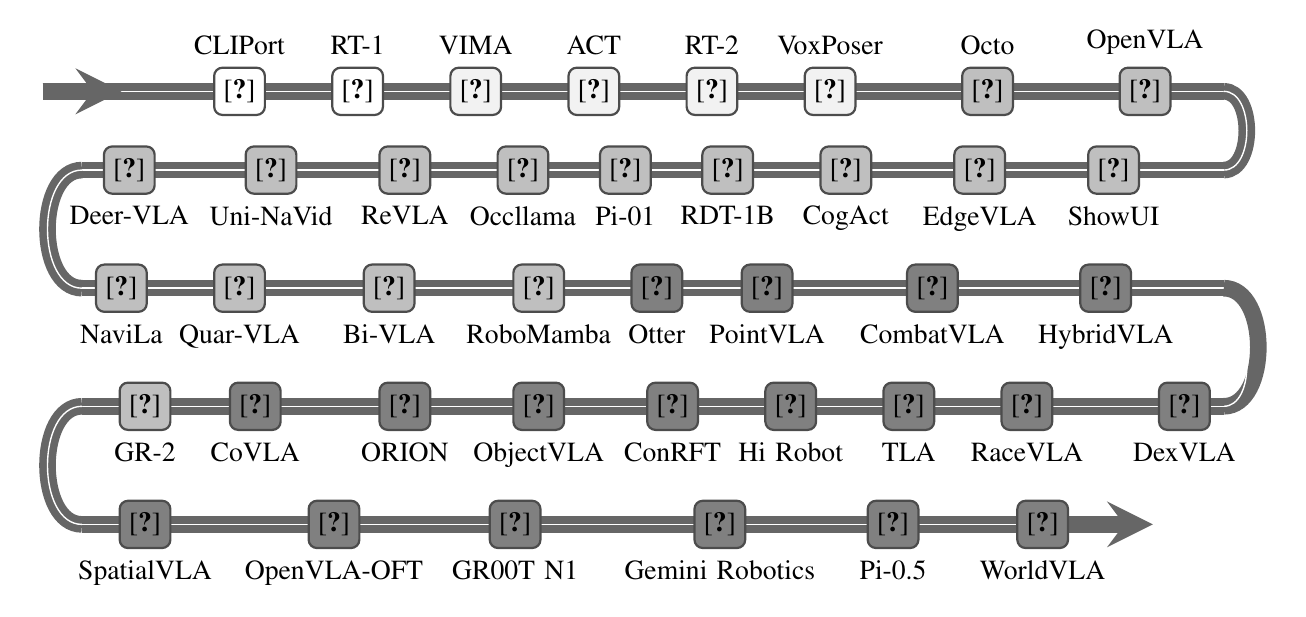
\begin{tikzpicture}[
  timeline/.style={ultra thick, draw=black!60, rounded corners=3pt},
    label/.style={align=center,  text width=2.3cm, inner sep=1pt},
    label2/.style={align=center,  text width=3cm, inner sep=1pt},
    event2022/.style={rounded corners=3pt, draw=black!70, fill=white, thick, minimum size=6mm, align=center, text=black},
    event2023/.style={rounded corners=3pt, draw=black!70, fill=gray!10, thick, minimum size=6mm,  align=center, text=black},
    event2024/.style={rounded corners=3pt, draw=black!70, fill=gray!50, thick, minimum size=6mm, align=center, text=black},
    event2025/.style={rounded corners=3pt, draw=black!70, fill=gray, thick, minimum size=6mm, align=center, text=black}
    ]

    % Main timeline path with reduced vertical spacing
    \draw[timeline,line width=6pt] (0,0) -- (15,0);
    \draw[-, line width=0.5pt, draw=white] (0,0) -- (15,0);
    % Arrow head at (0,0)
    \draw[-stealth, line width=6pt, draw=black!60] (0,0) -- (1,0);
    \draw[timeline,line width=6pt] (15,0) to[out=-0, in=0] (15,-1);
    \draw[-, line width=0.5pt, draw=white] (15,0) to[out=-0, in=0] (15,-1);
    \draw[timeline,line width=6pt] (15,-1) -- (0.5,-1);
    \draw[-, line width=0.5pt, draw=white] (15,-1) -- (0.5,-1);
    \draw[timeline,line width=6pt] (0.5,-1) to[out=-180, in=180] (0.5,-2.5);
    \draw[-, line width=0.5pt, draw=white] (0.5,-1) to[out=-180, in=180] (0.5,-2.5);
    \draw[timeline,line width=6pt] (0.5,-2.5) -- (15,-2.5);
    \draw[-, line width=0.5pt, draw=white] (0.5,-2.5) -- (15,-2.5);
    \draw[timeline,line width=6pt] (15,-2.5) to[out=-0, in=0] (15,-4);
    \draw[-, line width=0.5pt, draw=white] (15,-3) to[out=-0, in=0] (15,-4);
    \draw[timeline,line width=6pt] (15,-4) -- (0.5,-4); 
    \draw[-, line width=0.5pt, draw=white] (15,-4) -- (0.5,-4);
    \draw[timeline,line width=6pt] (0.5,-4) to[out=-180, in=180] (0.5,-5.5);
    \draw[-, line width=0.5pt, draw=white] (0.5,-4) to[out=-180, in=180] (0.5,-5.5);
    \draw[timeline,line width=6pt] (0.5,-5.5) -- (12.9,-5.5);
    \draw[-, line width=0.5pt, draw=white] (0.5,-5.5) -- (12.9,-5.5);
    \draw[-stealth, line width=6pt, draw=black!60] (12.9,-5.5) -- (14.1,-5.5);

    %%% Foundation Models %%%
    \node[event2022] (cliport) at (2.5,0) {\cite{shridhar2022cliport}};
    \node[label, above=3pt of cliport] {CLIPort};
    
    % \node[event2022] (gato) at (2.5,0) {\cite{reed2022generalist}};
    % \node[label, above=3pt of gato] {Gato};
    
    \node[event2022] (rt1) at (4,0) {\cite{rt-1}};
    \node[label, above=3pt of rt1] {RT-1};
    
    \node[event2023] (vima) at (5.5,0) {\cite{jiang2023vima}};
    \node[label, above=3pt of vima] {VIMA};
    
    \node[event2023] (act) at (7,0) {\cite{zhao2023learningFB}};
    \node[label, above=3pt of act] {ACT };
    
    \node[event2023] (rt2) at (8.5,0) {\cite{rt-2}};
    \node[label, above=3pt of rt2] {RT-2 };
    
    \node[event2023] (voxtposer) at (10,0) {\cite{huang2023voxposer}};
    \node[label, above=3pt of voxtposer] {VoxPoser };
    
    % \node[event2023] (diffpolicy) at (11.5,0) {\cite{chi2023diffusionpolicy}};
    % \node[label, above=3pt of diffpolicy] {Diffusion Policy };
    
    \node[event2024] (octo) at (12,0) {\cite{team2024octo}};
    \node[label, above=3pt of octo] {Octo };
    
    \node[event2024] (openvla) at (14,0) {\cite{kim2024openvla}};
    \node[label, above=3pt of openvla] {OpenVLA };

    %%% Specialized Applications %%%
    \node[event2024] (deer) at (1.1,-1) {\cite{yue2024deer}};
    \node[label, below=3pt of deer] {Deer-VLA };
    
    \node[event2024] (uni) at (2.9,-1) {\cite{zhang2024uni}};
    \node[label, below=3pt of uni] {Uni-NaVid };
    
    \node[event2024] (revla) at (4.6,-1) {\cite{dey2024revla}};
    \node[label, below=3pt of revla] {ReVLA };

    \node[event2024] (occllama) at (6.1,-1) {\cite{wei2024occllama}};
    \node[label, below=3pt of occllama] {Occllama };

    \node[event2024] (pi0) at (7.4,-1) {\cite{black2024pi_0}};
    \node[label, below=3pt of pi0] {Pi-01 };

    \node[event2024] (rdt) at (8.7,-1) {\cite{liu2024rdt}};
    \node[label, below=3pt of rdt] {RDT-1B };

    \node[event2024] (cogact) at (10.2,-1) {\cite{li2024cogact}};
    \node[label, below=3pt of cogact] {CogAct };

    \node[event2024] (edgevla) at (11.9,-1) {\cite{budzianowski20edgevla}};
    \node[label, below=3pt of edgevla] {EdgeVLA };

    \node[event2024] (showui) at (13.6,-1) {\cite{lin2024showui}};
    \node[label, below=3pt of showui] {ShowUI };

    %%% Robotics Focus %%%
    \node[event2024] (navila) at (1, -2.5) {\cite{cheng2024navila}};
    \node[label, below=3pt of navila] {NaviLa};

    \node[event2024] (quar) at (2.5, -2.5) {\cite{ding2024quar}};
    \node[label, below=3pt of quar] {Quar-VLA};

    \node[event2024] (bivla) at (4.4, -2.5) {\cite{gbagbe2024bi}};
    \node[label, below=3pt of bivla] {Bi-VLA};

    \node[event2024] (robomamba) at (6.3, -2.5) {\cite{liu2024robomamba}};
    \node[label, below=3pt of robomamba] {RoboMamba};

    \node[event2025] (otter) at (7.8, -2.5) {\cite{huang2025otter}};
    \node[label, below=3pt of otter] {Otter};

    \node[event2025] (pointvla) at (9.2, -2.5) {\cite{li2025pointvla}};
    \node[label, below=3pt of pointvla] {PointVLA};

    \node[event2025] (combatvla) at (11.3, -2.5) {\cite{chen2025combatvla}};
    \node[label, below=3pt of combatvla] {CombatVLA};

    \node[event2025] (hybridvla) at (13.5, -2.5) {\cite{liu2025hybridvla}};
    \node[label, below=3pt of hybridvla] {HybridVLA};

    %%% General Capabilities %%%
    \node[event2025] (covla) at (2.7, -4) {\cite{arai2025covla}}; % Changed from -6 to -5.2
    \node[label, below=3pt of covla] {CoVLA};
    % \node[event2025] (opendrivevla) at (2.7, -4) {\cite{zhou2025opendrivevla}}; % Changed from -6 to -5.2
    % \node[label, below=3pt of opendrivevla] {OpenDriveVLA};

    \node[event2025] (orion) at (4.6, -4) {\cite{fu2025orion}}; % Changed from -6 to -5.2
    \node[label, below=3pt of orion] {ORION};
    
    \node[event2025] (objectvla) at (6.3, -4) {\cite{zhu2025objectvla}}; % Changed from -6 to -5.2
    \node[label, below=3pt of objectvla] {ObjectVLA };

    \node[event2025] (conrft) at (8, -4) {\cite{chen2025conrft}}; % Changed from -6 to -5.2
    \node[label, below=3pt of conrft] {ConRFT};

    \node[event2025] (hirobot) at (9.5, -4) {\cite{shi2025hi}}; % Changed from -6 to -5.2
    \node[label, below=3pt of hirobot] {Hi Robot};

    \node[event2025] (tla) at (11, -4) {\cite{hao2025tla}}; % Changed from -6 to -5.2
    \node[label, below=3pt of tla] {TLA};
    
    \node[event2025] (racevla) at (12.5, -4) {\cite{serpiva2025racevla}}; % Changed from -6 to -5.2
    \node[label, below=3pt of racevla] {RaceVLA};

    \node[event2025] (dexvla) at (14.5, -4) {\cite{wen2025dexvla}}; % Changed from -6 to -5.2
    \node[label, below=3pt of dexvla] {DexVLA};
    %%% Newest Generalist Models (Q1--Q2 2025) %%%
    \node[event2024] (gr2) at (1.3, -4) {\cite{cheang2024gr2}};
    \node[label, below=3pt of gr2] {GR-2};

    \node[event2025] (spatialvla) at (1.3,-5.5) {\cite{qu2025spatialvla}};
    \node[label, below=3pt of spatialvla] {SpatialVLA};

    \node[event2025] (openvlaoft) at (3.7,-5.5) {\cite{openvla_oft}};
    \node[label2, below=3pt of openvlaoft] {OpenVLA-OFT};

    \node[event2025] (grootn1) at (6,-5.5) {\cite{gr00tn1}};
    \node[label, below=3pt of grootn1] {GR00T N1};

    \node[event2025] (geminirobotics) at (8.6,-5.5) {\cite{geminirobotics2025}};
    \node[label2, below=3pt of geminirobotics] {Gemini Robotics};

    \node[event2025] (pi05) at (10.8,-5.5) {\cite{pi05_2025}};
    \node[label, below=3pt of pi05] {Pi-0.5};

    \node[event2025] (worldvla) at (12.7,-5.5) {\cite{cen2025worldvla}};
    \node[label, below=3pt of worldvla] {WorldVLA};\end{tikzpicture}
}
\vspace{-4.4ex}
\caption{\small Recent robotic VLA models from {\fcolorbox{black}{white}{\small \text{2022}}} to {\fcolorbox{black}{gray}{\text{2025}}}.}\vspace{-1ex}
\label{fig:vla-timeline}
  \end{minipage}
  \vspace{-2ex}
\end{wrapfigure}
% {\vspace{-1ex}} 
\BfPara{End-to-end Robotic Learning}
Building generalist
robots advances in multiple dimensions: (1)
the development and integration of vision, language, large action models, and multimodal fusion techniques into robotic learning, 
(2) {\xo}-embodiment sensing and training using large, diverse datasets from across embodiments, enhanced transfer learning methods, and scalable data collection frameworks, and
(3) the incorporation of real-time feedback, reinforcement learning on modular robotic models for various tasks.
High-capacity models have demonstrated an exceptional ability to process and learn diverse and extensive datasets, which is critical for end-to-end robotic learning. 
These models leverage their vast parameter space, \eg GPT-3, Jurassic-1, WuDao-2 with 175B+, Microsoft and Nvidia's Megatron-Turing NLG with 530B, and Google's Switch Transformer with 1.56 trillion parameters, to capture intricate patterns and relationships within the data, enabling them to generalize effectively across a wide array of tasks. 
Compared to these models, models used for robotic learning directly are relatively smaller, \eg RT-1~\cite{rt-1}, MOO~\cite{stone2023open}, and CLIPort~\cite{shridhar2022cliport} (with CLIP-ViT-Base), have 35M+, 111M, and 400M+, respectively. RT-2~\cite{rt-2} and variations of RT-2-X~\cite{9} incorporate pre-trained VLMs, which have large parameter space (\eg RT-2-PaLM-E and RT-2-PaLI-X have 12B and 55B, respectively).
Scaling up these models faces many challenges: (1) maintaining real-time inference under strict time constraints (\eg 3-5Hz), (2) maintaining robustness and coherence when generalizing to novel tasks and environments, (3) addressing the computational demands and resource requirements of training and deployment, (4) managing the complexity of integrating multimodal inputs, and (5) ensuring reliability and safety in dynamic and unpredictable real-world settings.
As end-to-end techniques and integration of LLM and VLM backbones become more prevalent~\cite{9} (see the evolution of robotic models in \autoref{fig:vla-timeline}), security research for these models is limited. Generalist robotic models continue to emerge rapidly, with recent examples such as SpatialVLA, OpenVLA-OFT, {GR00T}~N1, Gemini Robotics, pi-0.5, and WorldVLA~\cite{qu2025spatialvla,openvla_oft,gr00tn1,geminirobotics2025,pi05_2025,cen2025worldvla,cheang2024gr2} added to \autoref{fig:vla-timeline}. Ensuring that these models are resilient to adversarial attacks is crucial and requires immediate attention.
To this end, we identify the following challenges.

\BfPara{C1: Wide-array of Data and Model Adoption}
The emergence of large-scale datasets for {\xo}-embodied generalist robots across diverse robotic platforms, embodiments, and environments has enabled many advances in the field.
Standardizing and processing these heterogeneous datasets in a consistent format requires substantial effort and innovation, as seen in efforts such as RoboNet~\cite{dasari2020robonet} and Open {\xo}-Embodiment Repository~\cite{9}. 
These datasets cover different kinds of tasks, objects, scenarios, and settings.
Moreover, recent work showed the benefits of learning visual representations from human video data~\cite{nair2022r3m,xiao2022masked,radosavovic2022,majumdar2024we,karamcheti2023language,mu2023ec2,bahl2023affordances} for robotics learning. 
Beyond robot-specific or {\xo}-embodied data/demonstrations, more and more data will inevitably be included in the pursuit of generalist robots.
This introduces new security and safety challenges that must be addressed to prevent/mitigate vulnerabilities.


\BfPara{C2: Multimodal Data and Model Integration} 
The integration of multimodal data, \ie vision, language, and action, into large foundation models for robotics presents substantial security complexities. 
Despite the importance of this integration to improve robot functionality and autonomy through understanding and interacting with unseen environments, the heterogeneous nature of multimodal data greatly increases the attack surface, offering multiple avenues for malicious interference. 
Each data modality introduces particular vulnerabilities; for instance, adversarial images can fool vision models, while subtly changed text inputs can fool language models. Moreover, it is more challenging to determine the impact of adversarial manipulations on input data due to the varied ways in which such data and models are used in end-to-end robot learning.
We must identify and counteract attacks that can exploit the specific weaknesses of each modality. 
%Constructing effective defense mechanisms that can adjust to new threats and work across different modalities is no easy feat.

\BfPara{C3: Robustness and Trustworthiness}
Ensuring the robustness and trustworthiness of robotic agents is a major challenge. %, particularly given the methods used to train policies for robotic agents. 
Few studies have adequately assessed factors such as interpretability, robustness, safety, and fairness in robots, raising concerns about the potential for inherited vulnerabilities and bias from large backbone models such as LLMs and VLMs. We must assess robot models
under a variety of conditions, including adversarial attacks and unexpected inputs, and develop methods that can improve their robustness.
We must develop methods for interpretability and fairness to ensure transparent and unbiased decisions.
%The complexity of training robotic policies, often involving reinforcement learning and continuous adaptation, complicates the assessment of these factors. 
%Without thorough evaluation, there is a risk that AI systems may inherit and propagate vulnerabilities from foundational models, compromising their safety and effectiveness. 

These challenges represent a tremendous opportunity for research into end-to-end learning models  for {\xo}-embodied generalist robots. 
The PI is an expert in AI security, especially in the security of large models. 
The PI has led significant work on secure and reliable AI systems~\cite{abuhamad2018large,abuhamad2020autosen,alasmary2020soteria,abuhamad2020multi,abusnaina2021dl,abuhamad2021large,abdukhamidov2023hardening,juraev2024unmasking,juraev2024impact,alawami2024motionid,abdukhamidov2024singleadv}, developing novel approaches to secure and interpretable AI \cite{abdukhamidov2023hardening,abusnaina2021dl,abdukhamidov2024singleadv,abdukhamidov2025stealthy,abuhamad2025nlp,abuhamad2025vit}, software security~\cite{abuhamad2018large,abuhamad2018large,abuhamad2020multi}, online security, privacy and safety~\cite{khan2023identification,reyes2023webtracker,shao2023lightweight,abuhamad2025shield}, and secure authentication methods~\cite{abuhamad2020autosen,alawami2024motionid}. 
These works appeared in ACM CCS, IEEE ICDCS, IEEE TDSC, ACM TOPS, IEEE TIFS, IEEE IoT-J, and PoPETS.  Because of this background and prior work, PI Abuhamad is uniquely positioned to carry out the proposed work.
The PI recognizes the vast and evolving landscape of adversarial attacks against large foundation models. 
In this project, over its four-year duration, the PI will work to establish foundational research and collaborative efforts to develop comprehensive frameworks and benchmarks that build toward secure and reliable robotic models. 
%While addressing all possible attack vectors is impossible within a single project, creating foundational tools, metrics, and methodologies will enable the broader research community to systematically evaluate and improve robotic system security. 
%The PI will leverage expertise in AI security to create lasting infrastructure that supports continuous improvement in robotic model security, with a particular focus on developing standardized evaluation protocols that can evolve alongside emerging threats.


\newpage
\section{Research Plan}

This work proposes a novel security framework for end-to-end generalist robots to address the inherent challenges of ensuring robustness, security, and trustworthiness in general-purpose robots across various physical embodiments. 
End-to-end generalist robot models leverage high-capacity models (\eg ViTs, LLMs, VLMs, and VLAs) pre-trained using Internet-scale data and training pipelines that use specific and/or \xot robotics datasets. 
The core concept relies on the systematic evaluation and discovery of potential vulnerabilities in all layers of the robotic learning stack. This plan describes the research tasks in this project.


\subsection{T0: Building Comprehensive Repository for End-to-end Robotic Models and Data}
% ~\vspace{-3ex}
\begin{wraptable}{r}{0.5\textwidth}\vspace{-3.5ex}
% \begin{table}
\centering
\caption{{Datasets augmenting OXE~\cite{9} for robots (\textbf{R}), \textbf{F}ranka, \textbf{G}oogle Robot, \textbf{S}pot, \textbf{H}ello Stretch, \textbf{U}R5, Hu\textbf{M}an}, and \textbf{X}arm7, with control frequency (\textbf{Hz}) and \textbf{\#} of episodes.}
\label{tab:multi_dataset}\vspace{-2ex}
\resizebox{0.99\linewidth}{!}{%
\begin{tabular}{lcclc}
\toprule
Dataset                     & \textbf{R}         &\textbf{ \#} & {Action Space}                           & \textbf{Hz}           \\
\midrule
 Franka  \cite{rosete2022tacorl,mees23hulc2}        & F       & 3242        & EEF Position                           & 15                            \\
Maniskill     \cite{gu2023maniskill2}               & F        & 30000       & EEF Position                           & 20                                               \\
Robocook   \cite{shi2023robocook}        & F       & 2460        & EEF Position                           & 5                                                \\
CMU Pick-Insert \cite{saxena2023multiresolution} & F        & 520         & EEF Position                           & 20                                      \\
RoboVQA  \cite{9}                       & G  & 61153       & EEF Position                           & 10                                                     \\
DROID \cite{khazatsky2024droid}                         & F        & 92233       & EEF Position                           & 15                                          \\
ConqHose  \cite{ConqHoseManipData}                     & S          & 139         & EEF velocity                           & 30                                          \\
DobbE   \cite{shafiullah2023dobbe}                     & H & 5208        & EEF Position                           & 3.75                                        \\
FMB \cite{luo2024fmb}                           & F        & 1804        & EEF velocity                           & 10                                                  \\
IO-AI Office \cite{9}    & M        & 3847        & EEF Position                           & 30                                                       \\
RoboSet\cite{bharadhwaj2023roboagent}                     & F        & 18250       & Joint position                         & 5                                        \\
VIMA \cite{jiang2023vima}                        & U          & 660103      & Primitive skills                       & NA                                               \\
SPOC \cite{spoc2023}                       & H & 233000      & Joint position                         & 10                                                     \\
Ours & X & 10000 & EEF/joint Position & 5-50 \\
\bottomrule
\end{tabular}}\vspace{-2ex}
\end{wraptable}
To conduct research tasks toward assessing and enhancing robustness, trustworthiness, and performance of robotic foundation models, we will build/train/evaluate various models using state-of-the-art techniques and \xot robotic data.\\
\BfPara{Robotics Data Mixture} We consider a multimodal robotics data mixture of
six robot embodiments (Franka, Google Robot, Spot, Hello Stretch, UR5, and Xarm7; \textit{fewer than the 22 embodiments in the OXE~\cite{9} dataset, for multimodality and practical reasons}) in addition to human demonstration data (see \autoref{tab:multi_dataset}). The mixture draws from 15 dataset sources: 14 robotics datasets (\autoref{tab:multi_dataset}, including our own for Xarm7) and the Open X-Embodiment (OXE)~\cite{9} repository, which itself aggregates 60 further robotic datasets.
% Freiburg Franka Play~\cite{rosete2022tacorl,mees23hulc2},
% Maniskill~\cite{gu2023maniskill2},
% Stanford Robocook~\cite{shi2023robocook},
% CMU Franka Pick-Insert Data~\cite{saxena2023multiresolution},
% RoboVQA~\cite{9},
% DROID~\cite{khazatsky2024droid},
% ConqHose~\cite{ConqHoseManipData},
% DobbE~\cite{shafiullah2023dobbe},
% FMB~\cite{luo2024fmb},
% IO-AI Office PicknPlace~\cite{9},
% RoboSet~\cite{bharadhwaj2023roboagent},
% VIMA~\cite{jiang2023vima},
% SPOC~\cite{spoc2023},
% and complemented by data taken from 
% RT-1~\cite{rt-1}, 
% QT-Opt~\cite{kalashnikov2018qt}, 
% Bridge~\cite{walke2023bridgedata}, 
% Jaco Play~\cite{dass2023jacoplay}, 
% Cable Routing~\cite{luo2023multistage}, 
% NYU VINN~\cite{pari2021surprising}, 
% Berkeley Autolab UR5~\cite{BerkeleyUR5Website}, 
% TOTO~\cite{zhou2023train} and 
% Language Table~\cite{lynch2023interactive} datasets.
% These datasets contain multiple modalities that are used to train RT-1-X and RT-2-X~\cite{9}.
% RT-1-X is trained on only the robotic data defined above, while RT-2-X is trained by co-fine-tuning (similarly to the original RT-2~\cite{rt-2}), with an approximately one-to-one split of the original VLM data and the robotics data mixture.
% Note, this data mixture includes data for 9 embodiments which is fewer than the entire OXE dataset (\ie 22) -- the practical reason for this difference is that we have continued to extend the dataset over time, and at the time of the experiments, the dataset above represented all of the data. In the future, 
We plan to continue extending our dataset (\ie added tasks and episodes) as we continue in our research and this project. 
% Other datasets, \ie for other embodiments, can and will be added to our repository when available to the research community.



\BfPara{End-to-end Models}
We identify two main families of end-to-end robotic foundation models: policy prediction models (\eg VLAs) and goal-conditioned models (\eg RoboCat~\cite{bousmalis2023robocat}). VLAs predict the next action based on the current state and instruction, while the second family, goal-conditioned models, predicts the next state based on the current state and goal. VLAs are gaining more traction due to their ability to leverage large pre-trained models and fine-tune them for specific tasks/embodiments (see~\autoref{fig:vla-timeline}).
{In the following, we describe the main models that we will use in this project. We will continue to expand the list of models as new models are released and/or become available for research use.}

\noindent\textbf{\cib{1} RT-1~\cite{rt-1} and RT-1-X~\cite{9}} RT-1 is a 35M parameter network built on a transformer architecture~\cite{vaswani2017attention} and designed for robotic control. %, as {shown} in~\autoref{fig:rtx}. 
It takes in a history of images (\eg 5 to 15 images) of resolution $300\times300$ along with the natural language instructions. 
Each image is processed through an ImageNet-pre-trained EfficientNet-B3~\cite{tan2019efficientnet} to output spatial feature maps of shape $9\times9\times512$ from the final convolutional layer.
The model was chosen primarily to balance accuracy, model size, and speed, keeping the local processing rate within 3Hz for the entire pipeline.
% \begin{wrapfigure}{r}{0.3\textwidth}{\vspace{-4.5ex}}
%   \centering
%   \includegraphics[width=0.29\textwidth]{figures/rt-1.pdf}\vspace{-2ex}
%       \caption{
%     \small RT-1-(X) and RT-2-(X) variations for {\xo}-embodied robotics.
%     }\vspace{-2ex}
%   \label{fig:rtx}
% \end{wrapfigure}
The natural language instruction is transformed into a USE~\cite{cer2018universal} embedding. 
The visual and language representations are then interwoven via FiLM~\cite{perez2017film} layers, producing 81 vision-language tokens. 
These tokens are fed into a decoder-only transformer that outputs the tokenized actions.
To tokenize actions, each action dimension in RT-1 is discretized into $256$~bins. 
The action dimensions we consider include seven variables for the arm movement ($x$, $y$, $z$, roll, pitch, yaw, opening of the gripper), three variables for base movement ($x$, $y$, yaw), and a discrete variable to switch between three modes: controlling arm, base or terminating the episode.
For example, an action
``$\Delta \textit{pos}_x\text{=}0.1 \enspace \Delta \textit{pos}_y\text{=}-0.2 \enspace \Delta \textit{pos}_z\text{=}0 \enspace \Delta \textit{rot}_x\text{=}10^{\circ} \enspace \Delta \textit{rot}_y\text{=}25^{\circ} \enspace \Delta \textit{rot}_z\text{=}-7^{\circ}
$'' for the arm could be represented as ``\textit{132 114 128 5 25 156}''.
For each variable, the target action/value is mapped to a value from the 256 bins, where the bins are uniformly distributed within the bounds of each variable. The {loss}
used for RT-1 training is a standard categorical cross-entropy entropy and causal masking that was utilized in prior transformer-based controllers~\cite{reed2022generalist,lee2022multi}. 
We use the same implementation/design choices for RT-1 model as reported by the original work. Other variations of RT-1, \eg different base/backbone models and operation modes (\ie local or cloud-based inference), will be implemented as RT-1-X designs.


\noindent\textbf{\cib{2} RT-2~\cite{rt-2} and RT-2-X~\cite{9}} RT-2 is a large (12--55B parameters) VLA model trained on Internet-scale vision and language data, along with robotic control data. 
RT-2 casts the tokenized actions as text tokens.
As such, any pre-trained VLM (\eg Pali-X~\cite{chen2023palix}, Flamingo~\cite{alayrac2022flamingo}, {P}a{LM}-E~\cite{driess2023palme}) can be fine-tuned for robotic control, thus leveraging the backbone of VLMs and transferring some of their generalization properties.
Action encoding and discretization are performed as in \cite{rt-1} for the RT-1 model. 
To fine-tune a VLM into a VLA model, tokens should be associated with the discrete action bins (\ie reserving 256 tokens to serve as action tokens). 
In order to define a target for VLM fine-tuning, the action vector is represented by a single string that simply concatenates action tokens for each dimension with a space character:
For example, a possible instantiation of the target,
``$\textit{terminate} \enspace \Delta \text{pos}_x \enspace \Delta \textit{pos}_y \enspace \Delta \textit{pos}_z \enspace \Delta \textit{rot}_x \enspace \Delta \textit{rot}_y \enspace \Delta \textit{rot}_z \enspace \textit{gripper\_extension}
$'',
could be: ``\textit{1 128 91 241 5 101 127}''.
To ensure that RT-2 outputs valid action tokens during decoding, the output vocabulary is
constrained to only sampling valid action tokens when the model is prompted with a robot-action task.
We note that the model, \ie the orginal VLM, can still output the full range of language tokens on standard vision-language tasks.
Our implementation focuses on the RT-2-PaLI-X variants~\cite{chen2023palix} built on the backbone of ViT~\cite{dosovitskiy2021image} visual model and UL2~\cite{tay2023ul2} language model, and pre-trained on WebLI~\cite{chen2023palix} dataset. %Variations of RT-2 will be implemented as RT-2-X designs for \xod training.

\begin{wraptable}{r}{0.5\textwidth}
\centering
\vspace{-2ex}
\caption{{\small Possible VLMs (and variations) for RT-2-X.}}
\label{tab:VLMs}
\vspace{-2ex}
\scalebox{0.73}{
\begin{tabular}{llll}
\toprule
Model & LLM & Adapter & Vision \\ \midrule
Flamingo~\cite{alayrac2022flamingo} & Chinchilla & Attention & NFNet-F6 \\
OpenFlamingo~\cite{awadalla2023openflamingo} & MPT & Attention & CLIP ViT-L \\
SPHINX-X~\cite{gao2024sphinx} & Mixtral & Linear & Mixture \\
Qwen-VL~\cite{bai2023qwen} & Qwen & Q-Former & ViT-bigG \\
BLIP-2~\cite{li2023blip} & Flan-T5/OPT & Q-Former & EVA ViT-g \\
InstructBLIP~\cite{dai2024instructblip} & Vicuna & Q-Former & EVA ViT-g \\
BLIVA~\cite{hu2024bliva} & Vicuna & Q-Former & EVA ViT-g \\
MiniGPT-4~\cite{zhu2023minigpt} & Vicuna & Linear & EVA ViT-g \\
MiniGPT-v2~\cite{chen2023minigpt} & LLaMA-2 & Linear & EVA ViT-g \\
LLaVA~\cite{liu2024visual} & Vicuna & Linear & CLIP ViT-L \\
LLaVA-1.5~\cite{liu2024improved} & Vicuna-v1.5 & MLP & CLIP ViT-L \\
LLaMA Adapter-V2~\cite{gao2023llama} & LLaMA & Linear & CLIP ViT-L \\
PandaGPT~\cite{su2023pandagpt} & Vicuna & Linear & ImageBind \\
\bottomrule
\end{tabular}}\vspace{-2ex}
\end{wraptable}
We will explore the adoption of other existing VLMs in the RT-2-X implementation for \xod training. 
\autoref{tab:VLMs} lists common open-source VLMs along with their respective components.
Typically, a VLM is composed of three key elements: a visual encoder (\ie vision model), an adapter, and an LLM backbone. 
The visual encoder extracts visual features from the input images, facilitating subsequent LLM reasoning and understanding of visual semantics. 
The most used visual encoders are pre-trained ViT models, with popular choices including the ViT-L model from CLIP \cite{radford2021learning} and the ViT-g from EVA-CLIP \cite{fang2023eva}. 
In addition to ViT-based models, other approaches employ ImageBind \cite{girdhar2023imagebind} and NFNet-F6 \cite{brock2021high}, among others, as visual encoders.
The adapter module connects the visual and textual input modalities. 
VLMs use various adapters, from basic architectures such as linear layers and MLPs to advanced ones such as Q-Former \cite{li2023blip} and cross-attention \cite{vaswani2017attention}.
For the LLM component, the LLaMA family is commonly preferred as the LLM backbone, primarily due to its open source status and the range of versions available to suit different requirements/capacities, such as LLaMA \cite{touvron2023llama}, LLaMA-2 \cite{touvron2023llama2}, Vicuna, and Vicuna-v1.5 \cite{chiang2023vicuna}. 
Other LLM backbones include Flan-T5 \cite{chung2024scaling}, MPT \cite{mosaicml2023introducing}, Chinchilla \cite{hoffmann2022training}, OPT \cite{zhang2022opt}, Mixtral \cite{jiang2024mixtral}, and Qwen \cite{bai2023aqwen}. 
We plan to explore variations of VLMs in building RT-2-X and evaluate the impact of architecture design on the development of robotic models. %Similarly, multiple vision models with the RT-1-X design will be evaluated.

% \noindent\textbf{\cib{3} } Variants of RT-1 and RT-2 with different base/backbone models will be implemented to assess the impact of design choices on performance and robustness of models. In addition, we will evaluate the impact of incorporation of various datasets, including \xot datasets, on the generalization, performance, and robustness of models.
% We note that other implementations of generalist robotic models, \eg ~{MOO}~\cite{stone2023open} will be included in our evaluation. {MOO}~\cite{stone2023open} employs a VLM to generate an additional image channel for a semantic map, which is subsequently fed into an RT-1 backbone.

\noindent\textbf{{\cib{3}} OpenVLA and [X]-VLA Variants} 
OpenVLA~\cite{kim2024openvla} (7B parameters)
is an open-source alternative to RT-2~\cite{rt-2}. % that is built on the open-source VLMs.
OpenVLA, as other VLAs, follows the same design principles that include training/fine-tuning open-source VLMs which consist of three components: vision tokenizer/encoder/adapter, LLM backbone, and action decoder/tokenizer. 
OpenVLA uses Prismatic VLM (7B-parameter) and is trained on 970k real-world robot demonstrations outperforming larger models like RT-2 ($\sim$55B). The Prismatic VLM uses dual vision encoders (DINOv2 \cite{oquab2023dinov2} and SigLIP \cite{zhai2023sigmoid}) and a LLaMA-2 language model \cite{touvron2023llama}.
Variants of OpenVLA, \eg  ReVLA~\cite{dey2024revla}, Edge-VLA~\cite{budzianowski20edgevla}, PointVLA~\cite{li2025pointvla}, and CoVLA~\cite{arai2025covla} (see \autoref{fig:vla-timeline}), have been proposed to improve the original design in terms of performance, efficiency, reasoning, and/or specialty.
Similar to RT-2-X, we will adopt various open-source VLMs/components (in \autoref{tab:VLMs}) to build/train [X]-VLA variants.


\noindent\textbf{\cib{4} RoboCat~\cite{bousmalis2023robocat}} RoboCat follows a different approach by conditioning the model on visual goal. The architecture is VQ-GAN encoder which is based on the Gato architecture~\cite{esser2021taming} that processes the image (with $128\times128$ resolution) as $8\times8$ tokens and outputs encoded vectors. These vectors are then discretized via a nearest-neighbor lookup in a codebook of embeddings.
The VQ-GAN encoder is a ResNet~\cite{resnet} with 2 groups of 2 blocks, followed by 3 attention layers. 
The decoder has 3 attention layers followed by a ResNet with 2 groups of 3 blocks. %The vector quantiser~\citep{van2017neural} uses 64 embeddings of dimension 128. 
For tokenization of observations and actions, RoboCat follows a similar approach as~\cite{reed2022generalist}.
The loss is weighted as ($0.25\times\text{discretization\_loss} + \text{l2\_reconstruction\_loss} + 0.1\times\text{log\_laplace\_loss}$) to predict future tokens. The output is the image tokens at time step $k = 5$, as one step can look very similar.

\noindent\textbf{\cib{5} Octo~\cite{team2024octo}} Octo is a (27-93M parameters) transformer-based VLA pre-trained on the OXE~\cite{9} dataset. Unlike RT-X and RoboCat, it can be fine-tuned to new observations and action spaces. This flexibility allows Octo to adapt to various robotic embodiments, a trend that is becoming increasingly important/adopted in robotics.
Octo architecture consists of three key parts: \textit{input tokenizers} that transform language instructions and observations into tokens, a \textit{transformer backbone} that receives the tokens and generates embeddings, and \textit{readout heads} that produce the desired outputs, \ie actions. Input tokenizers include modality-specific tokenizers, \ie a language (task) tokenizer (\eg T5) and a vision tokenizer (\eg ViT-based or CNN-based). Unavailable modalities are masked (\eg no language instructions are provided), and learnable position embeddings are added to the input tokens before feeding them into the transformer backbone.  Octo also uses a \textit{readout token} analogous to the $\text{[CLS]}$ token in BERT/LLMs.
The transformer backbone processes the input tokens through block-wise masked attention patterns (\ie see to tokens from the same or earlier time steps), which are then passed to the readout heads. The readout ``\textit{action}'' head predicts a ``\textit{chunk}'' of several consecutive actions.
Action heads can be added/replaced/fine-tuned during downstream fine-tuning (\eg adoption of new embodiments).


\noindent\textbf{\cib{6} ACT~\cite{zhao2023learningFB}} ACT is a VLA model that uses ResNet~\cite{resnet} as the vision encoder and transformer-based
conditional variational autoencoder (CVAE)~\cite{sohn2015learning} that generates a sequence of actions. The original ACT 
\begin{wrapfigure}{r}{0.45\textwidth}{\vspace{-2ex}}
  \centering
\begin{minipage}{0.45\textwidth}
      \centering
        \begin{minipage}{\linewidth}
          \centering
          \begin{minipage}{0.33\linewidth}
            \centering
            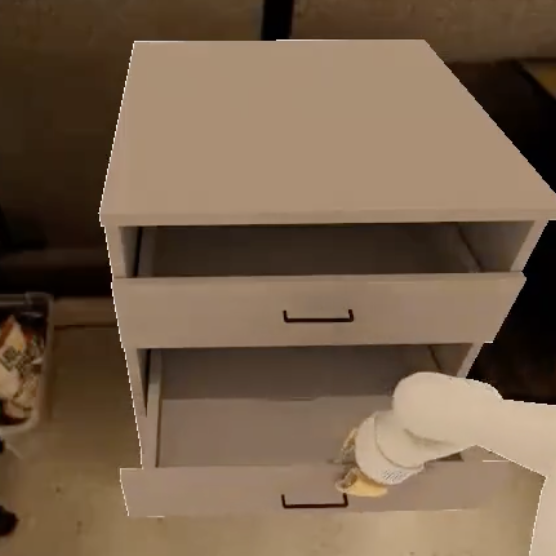
\includegraphics[width=\textwidth]{figures/examples/1.png}
          \end{minipage}%
          \begin{minipage}{0.33\linewidth}
            \centering
            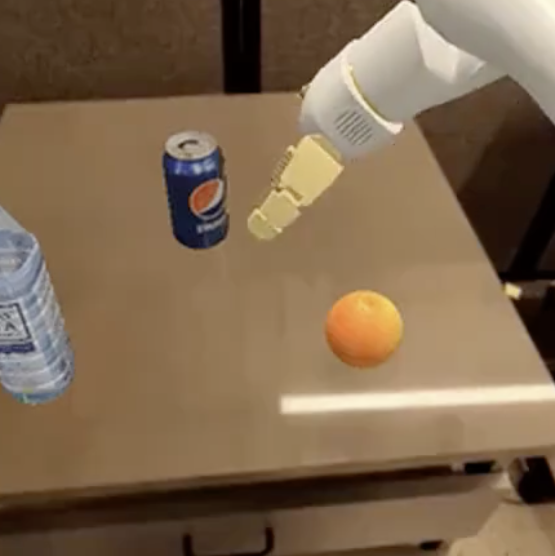
\includegraphics[width=\textwidth]{figures/examples/2.png}
          \end{minipage}%
          \begin{minipage}{0.33\linewidth}
            \centering
            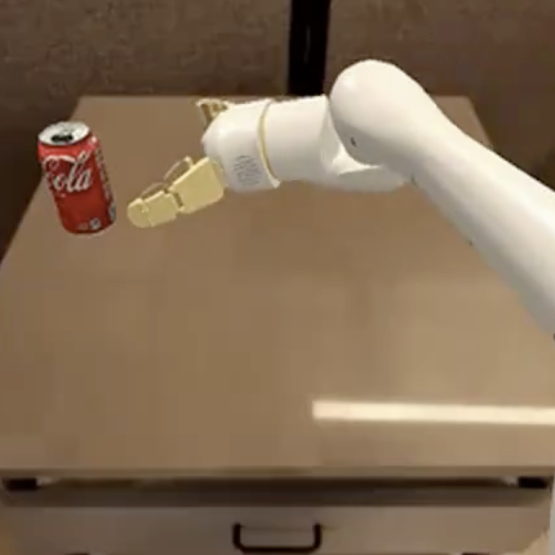
\includegraphics[width=\textwidth]{figures/examples/3.png}
          \end{minipage}
        \end{minipage}\vspace{-1.5ex}
        \begin{minipage}{\linewidth}
          \centering
          \begin{minipage}{0.33\linewidth}
            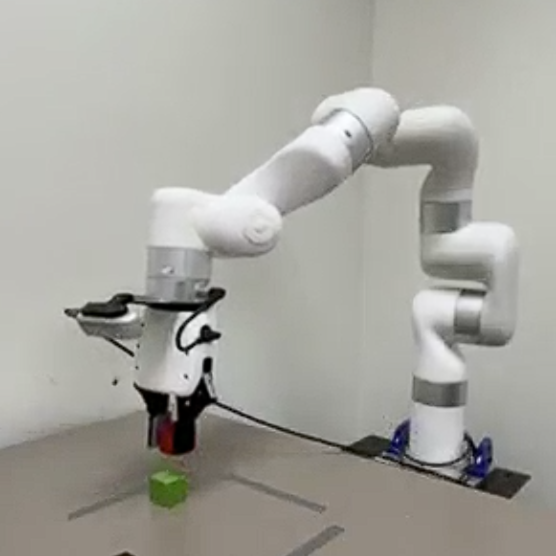
\includegraphics[width=\textwidth]{figures/examples/4.png}
          \end{minipage}%
          \begin{minipage}{0.33\linewidth}
              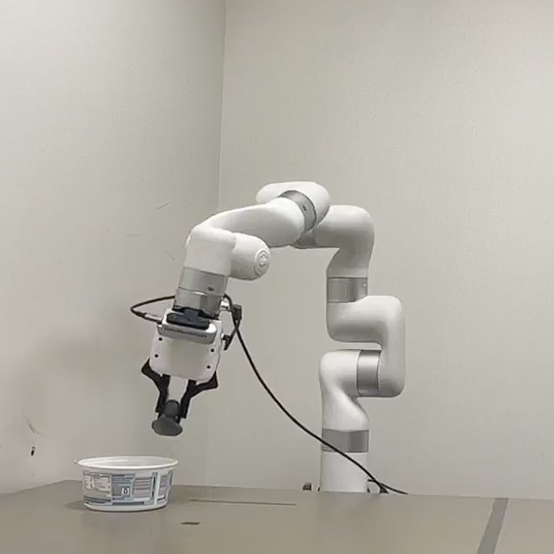
\includegraphics[width=\textwidth]{figures/examples/5.png}  
            \end{minipage}%
          \begin{minipage}{0.33\linewidth}
            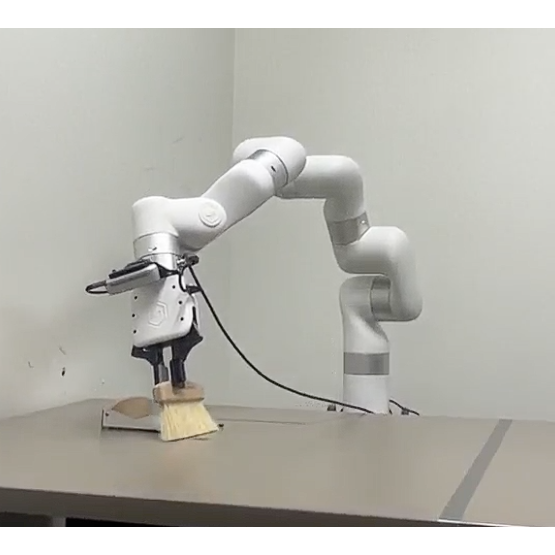
\includegraphics[width=\textwidth,trim={10pt 0 50pt 0},clip]{figures/examples/6.png}
          \end{minipage}\vspace{-2.5ex}
          \caption{\textbf{(Top)} Simulation tasks from Simpler~\cite{li24simpler}: {Close drawer}, {Move closer}, and {Pick Coke Can}. \textbf{(Bottom)} 
          Xarm7: {Stack Cubes}, {Duck in Bowl}, and {Sweep}.}
          \label{fig:xarm7}
        \end{minipage}
    \end{minipage}%
  \hfill
    \begin{minipage}{0.45\textwidth}
      \centering
      \begin{minipage}{0.45\linewidth}
        \centering
        \includegraphics[width=\textwidth]{figures/results/sim_res.pdf}
      \end{minipage}
      \hfill
      \begin{minipage}{0.49\linewidth}
        \centering
        \includegraphics[width=\textwidth]{figures/results/real_res.pdf}
      \end{minipage}
      \vspace{-2.5ex}
      \caption{Performance of models on simulated (left) and real (right) robotic tasks.}
      \label{fig:res}
    \end{minipage}\vspace{-2ex}
\end{wrapfigure}
was designed to process visual data and joint positions without additional language instructions. 
Similar to Octo~\cite{team2024octo}, ACT processes the images (multiple views if available, \eg original ACT uses 4 camera views) through a ResNet model, adds positional embeddings, and feeds them into a transformer-based CVAE-encoder (along with joint positions) to generate a sequence of actions (projected using MLP to chunks of absolute joint positions) through the CVAE-decoder.
For example, for Bimanual robots, the observation includes 4 RGB images (4 cameras), each at $480\times640$ resolution, and joint positions for two robot arms (7+7=14 positions in total).
The ResNet processes each image ($480\times640\times3$) and outputs feature maps of 4 images $\times$ $15\times20\times512$.
These feature maps are flattened ($1200\times512$), added to positional embeddings, and fed into the transformer encoder with additional joint position information.
The transformer decoder processes the encoder output through cross-attention to generate a sequence of actions ($k \times 512$ where $k$ is the number of action chunks). To generate the final actions, the output is down-projected with an MLP to $k \times 14$ dimensions, corresponding to the target joint positions for the next $k$ steps.
Our implementation of ACT will follow the original design choices, but changes are adopted to accommodate data from other embodiments, which can change the number of views and action dimensions, \eg the Xarm7 robot has 1 camera view (additional views can be added) and 7 action dimensions (7 degree-of-freedom positions).






\BfPara{Preliminary Experiments: Robotic Models} 
We have conducted preliminary experiments to evaluate the performance of robotic models, \ie RT-1, RT-2, Octo, and ACT on simulated and real robotic tasks. 
For simulation, we used Simpler~\cite{li24simpler} benchmark for three tasks: \emph{Close the drawer}, \emph{Move closer}, and \emph{Pick the Coke Can} using Google robot embodiment, while for real experiments, we used Xarm7 robot for three tasks: \emph{Stack Cubes}, \emph{Duck in Bowl}, and \emph{Sweep} (see~\autoref{fig:xarm7}).
For the simulation tasks, models were fine-tuned (using single third-person view and language-conditioned control) using 50 episodes per task. Language instructions are not used for ACT. Five training runs were performed per model, where each run was trained for 20,000 iterations with a batch size of 512 and a learning rate of 1e-5 using AdamW optimizer. The evaluation was performed on 25 episodes per task over five runs with different random seeds.
Similar training and evaluation settings were used for the real robotic tasks, but with visual observations only and no language instructions to avoid any changes on the ACT model architecture. 
Task success is measured using a two-point scoring system. For \emph{Stack Cubes} (stacking two cubes) and \emph{Duck in a bowl} (placing duck in bowl), points are awarded for successful pick (1 point) and place (1 point) operations. For \emph{Sweep}, points are given for finding (1 point) and sweeping objects into the bin (1 point). The success rate is calculated as the average scores divided by the total points in all evaluation episodes.
The preliminary results are shown in~\autoref{fig:res}.

% \BfPara{Adoption and Constraints}
% At inference time, each model is required to run at the rate required for the robot (3-10~Hz). 
% While relatively small models, \eg ACT, Octo, RT-1 can run locally on some robots with such inference rate, larger models, \eg OpenVLA and RT-2 (7B+ parameters), are hosted on a cloud service and queried over the network. This can introduce latency and network reliability issues, which are critical for real-time robotic applications.
% Even when designing/training such models to generate chunks of actions at once, which can be executed over several time steps,
% robotic models require strict real-time performance for smooth operation. % unlike general LLM/VLMs which often operate without stringent timing constraints.
% This adds complexity to robotic models, \ie managing latency, network reliability, and data communication security aspects that are less critical in typical LLM/VLM applications.
% In terms of adversarial attacks, attacking a robot's availability through prompt injection or jailbreak attacks (\eg running prompts that take more than 15Hz) can have far more serious consequences than similar attacks on other LLM/VLM applications.
% Compromised availability (and/or functionality) of a robot from an attack can cause physical harm, property damage, or operational disruptions.
% The real-time and/or (network dependence) of these models adds vulnerabilities that can be exploited to disrupt availability, making it imperative to prioritize security and resilience against such attacks.




\subsection{T1: Vulnerability Analysis in Foundation Generalist Robots}

This task aims to secure emerging robotic foundation models, where security and robustness are crucial.
Vulnerabilities in AI models have been the focus of many studies recently, showing how small adversarial manipulations to the model's input can significantly impact their performance.
Adversarial machine learning has emerged as an active field of research that addresses various threats to AI systems.
Based on the NIST Trustworthy and Responsible AI report~\cite{NIST_AI_100_2e2023}, the taxonomy of the most studied and effective attacks includes \emph{evasion}, \emph{poisoning}, and \emph{privacy} attacks for predictive AI systems with the addition of \emph{abuse} attacks for generative AI systems.
Since end-to-end robotic models fall into the generative AI category, this task addresses all categories of attacks, including evasion, poisoning, privacy, and abuse attacks.
% Given the high-dimensional and multimodal nature of the search space for attacks aginst robotic models, simply introducing random noise to inputs might fail to identify subtle vulnerabilities of the robotic model.
% Moreover, robotic models/policies are generally designed to be resilient against such noise~\cite{miki2022scirob}, making such adversarial attacks ineffective using straightforward methods.







\BfPara{Challenges in Attacking Robotic Models} 
Attacking robotic models
presents unique challenges due to their complex architectures, the multimodal nature of their input, restrictions on the output/action space, and the evolving landscape of security measures. 
Understanding these challenges is crucial for developing effective attack strategies that help
uncover vulnerabilities and improve the robustness of these models. 
Main challenges include the following:
{\cib{1}} \textbf{{Multimodal Complexity}}: Generalist robotic models process/integrate data from multiple modalities, such as sensory/positions data, images, and text, to predict action sequences. We believe that the efforts to build robotic foundation models will continue to grow and other modalities will be incorporated.
    Creating effective attacks requires understanding and manipulating the intricate relationships and interactions among these modalities \cite{radford2021learning}. 
    Consequently, creating adversarial examples that can deceive both the visual and language components is more challenging than focusing on one. %, such as attacks on vision models~\cite{abdukhamidov2023hardening,abdukhamidov2024singleadv} and LLM~\cite{chowdhury2024breaking}, or unimodal attacks VLM \cite{fan2024unbridled}.
\\{\cib{2}} \textbf{{Model Scale and Complexity}}: Current end-to-end robotic models involve large architectures containing millions to billions of parameters, making them highly complex and computationally expensive to attack.
    Adapting traditional adversarial attacks from downstream tasks to successfully impact such large models necessitates significant computational resources and sophisticated optimization methods.
\\{\cib{3}} \textbf{{Attack Practicality and Transferability}}: 
    Adversarial scenarios against robotics should be practical, \ie scenarios in which robots are likely to face operational tasks. 
Therefore, attacks must be systematic and guided by practical experience in field robotics to ensure the plausibility and reflection of real-world scenarios. 
    Moreover, attack methods against similar LLMs/VLMs use white-, gray-, and black-box settings relying on prior knowledge of (exact or similar) models, training data, restrictions/constraints of the system or training a surrogate models. However, robotic applications and commercial vendors often do not share model details \cite{cheng2018query}. In practice, attackers can only query the model and observe the behavior of the robot/output of the model. Developing attacks that exploit multiple vulnerabilities \cite{biggio2018wild} or adapt to various threat vectors is necessary and requires versatile strategies.
    Moreover, an effective attack should be undetectable/imperceptible by human/robot observer, which requires preserving the semantic traits of the benign sample. 
    This requires well-designed constraints to restrict the type and size of the perturbation. 
    Numerous studies have shown that some attacks inhibit high transferability, \ie attacks on a given model can succeed on other similar models. This phenomenon derived the transfer-based black-box attacks.
    Nevertheless, attacks designed for similar LLMs/VLMs models might not always work effectively on other models, even if they share similar architectures. 
    Ensuring adversarial examples are transferable \cite{liu2016delving} across models and tasks requires understanding model-specific vulnerabilities and generalizable attack methods.





        % Highly improbable conditions, like disturbances significantly beyond normal environmental challenges, do not contribute effectively to our understanding of a controller's nuanced vulnerabilities. 
    
    %\item  \textbf{Interpretable and Explainable Attacks}: For attacks to be truly effective, attackers need to understand the internal workings and decision-making processes \cite{doshi2017towards} of VLMs. However, the black-box nature of many VLMs, coupled with their complexity, makes it difficult to interpret how and why an attack succeeds or fails.
    % \item  \textbf{Robustness to Defenses}: Many VLMs incorporate dynamic defense mechanisms that can adapt to detected adversarial activities. These defenses may include real-time monitoring, anomaly detection, and adaptive retraining. Therefore, attack strategies need to continuously evolve to stay ahead of these adaptive defenses, which require substantial computational resources and sophisticated algorithms.






\BfPara{Attacking Robotic Foundation Models}
~{Let $\mathcal{M}$ represent a robotic foundation model, which takes a tuple of inputs, \eg $(\{\bm{x}\}, \{\bm{t}\}, \{\bm{s}\}, \dots)$ representing input modalities (\ie a set (at least one) of images \{$\bm{x}\} \in \mathcal{X}$, set of text instructions \{$\bm{t}\} \in \mathcal{T}$, set of sensory/position data $\{\bm{s}\}\in \mathcal{S}$, and other available information) and outputs a set of tokenized actions $\mathcal{M}(\{\bm{x}\}, \{\bm{t}\}, \{\bm{s}\}, \dots)=\{\bm{a}_{out}\}$.
Since robots could have multiple embodiments/tasks (and various action spaces), some inputs could become a placeholder/masked $\oslash$ or nonexistent modified to fit the model.}
%%{\vspace{-2ex}}
% Let $\mathcal{M}$ represent a robotic foundation model, which takes a tuple of inputs, \eg $(\{\bm{x}\}, \{\bm{t}\}, \{\bm{s}\}, \dots)$ representing input modalities (\ie a set (at least one) of images \{$\bm{x}\} \in \mathcal{X}$, set of text instructions \{$\bm{t}\} \in \mathcal{T}$, set of sensory/position data $\{\bm{s}\}\in \mathcal{S}$, and other available information) and outputs a set of tokenized actions $\mathcal{M}(\{\bm{x}\}, \{\bm{t}\}, \{\bm{s}\}, \dots)=\{\bm{a}_{out}\}$.
% Since robots could have multiple embodiments/tasks (and various action spaces), some inputs could become a placeholder/masked $\oslash$ or nonexistent modified to fit the model.
For example, RT-2 and OpenVLA models receive only images and textual instruction $\mathcal{M}(\{\bm{x}\}, \{\bm{t}\})=\bm{a}_{out}$, 
%RoboCat and RT-1 receive images and no text, $\mathcal{M}(\{\bm{x}\}, \oslash)=\bm{a}_{out}$, 
Octo receives images, text, and sensory data $\mathcal{M}(\{\bm{x}\}, \{\bm{t}\}, \{\bm{s}\})=\bm{a}_{out}$, and ACT receives only images and sensory data $\mathcal{M}(\{\bm{x}\}, \{\bm{s}\})=\bm{a}_{out}$.
If Octo is used for robots/datasets that do not provide text instructions, the model processes available inputs and mask unavailable ones $\mathcal{M}(\{\bm{x}\}, \oslash,\{\bm{s}\})=\bm{a}_{out}$.
The output $\{\bm{a}_{out}\}$ is one or chunks of actions, each is a sequence of tokens representing predicted actions.



The attack operation $\mathcal{P}(.)$ is defined as a perturbation function that alters the inputs (one or more 
\begin{wraptable}{r}{0.5\textwidth}
\centering \vspace{-2ex}
\caption{{\small Stages (Training and Inference), targets (Privacy, Integrity, Availability, and Abuse) and types ( White- (\dd), Gray- (\bb), and Black-box (\vv) ) of common Evasion, Poisoning, and Privacy attacks.}}\vspace{-3.5ex}
\label{table:attacks_models}
\small
\resizebox{0.98\linewidth}{!}{%
\begin{tblr}{
rowsep=0pt,
  column{3} = {c},
  column{4} = {c},
  column{5} = {c},
  column{6} = {c},
  column{7} = {c},
  column{8} = {c},
  column{9} = {c},
  cell{2}{1} = {r=7}{},
  cell{10}{1} = {r=10}{},
  cell{20}{1} = {r=6}{},
  hline{2,10,20,26} = {-}{},
}
                                                  &                                & \begin{sideways}Training\end{sideways} & \begin{sideways}Inference\end{sideways} & \begin{sideways}Privacy\end{sideways} & \begin{sideways}Integrity\end{sideways} & \begin{sideways}Availability\end{sideways} & \begin{sideways}Abuse\end{sideways} & \begin{sideways}Type\end{sideways} \\
\begin{sideways}Evasion      ~\end{sideways}      & Indirect Prompt Injection      & \ee                                       & \checkmark                                         & \checkmark                                       & \checkmark                                         & \checkmark                                            & \checkmark                                     & \vv                          \\
                                                  & Universal Adversarial Triggers & \ee                                       & \checkmark                                         & \ee                                      & \ee                                        & \ee                                           & \checkmark                                     & \vv                          \\
                                                  & Gradient-based Attacks         & \checkmark                                        & \checkmark                                         & \ee                                      & \ee                                        & \ee                                           & \ee                                    & \dd                          \\
                                                  & Prompt Injection               & \ee                                       & \checkmark                                         & \checkmark                                       & \checkmark                                         & \checkmark                                            & \checkmark                                     & \bb                           \\
                                                  & Refusal Suppression            & \ee                                       & \checkmark                                         & \ee                                      & \ee                                        & \ee                                           & \checkmark                                     & \bb                           \\
                                                  & Style Injection                & \ee                                       & \checkmark                                         & \ee                                      & \ee                                        & \ee                                           & \checkmark                                     & \bb                           \\
                                                  & Role-play Strategies           & \ee                                       & \checkmark                                         & \ee                                      & \ee                                        & \ee                                           & \checkmark                                     & \bb                           \\
                                                  & Jailbreak           & \ee                                       & \checkmark                                         & \ee                                      & \ee                                        & \ee                                           & \checkmark                                     & \bb                           \\
\begin{sideways}Poisoning         ~\end{sideways} & Data Poisoning                 & \checkmark                                        & \ee                                        & \ee                                      & \checkmark                                         & \checkmark                                            & \ee                                    & \dd                          \\
                                                  & Model Poisoning                & \checkmark                                        & \ee                                        & \ee                                      & \checkmark                                         & \checkmark                                            & \ee                                    & \dd                          \\
                                                  & Backdoor Poisoning             & \checkmark                                        & \checkmark                                         & \checkmark                                       & \ee                                        & \ee                                           & \checkmark                                     & \dd                          \\
                                                  & Label Flipping                 & \checkmark                                        & \ee                                        & \ee                                      & \checkmark                                         & \checkmark                                            & \ee                                    & \dd                          \\
                                                  & Clean-label Poisoning          & \checkmark                                        & \ee                                        & \ee                                      & \ee                                        & \ee                                           & \ee                                    & \dd                          \\
                                                  & Targeted Poisoning             & \checkmark                                        & \ee                                        & \ee                                      & \ee                                        & \ee                                           & \ee                                    & \dd                          \\
                                                  & Subpopulation Poisoning        & \checkmark                                        & \ee                                        & \ee                                      & \ee                                        & \ee                                           & \ee                                    & \dd                          \\
                                                  & Model Replacement              & \checkmark                                        & \ee                                        & \ee                                      & \ee                                        & \ee                                           & \ee                                    & \dd                          \\
                                                  & Model Boosting                 & \checkmark                                        & \ee                                        & \ee                                      & \ee                                        & \ee                                           & \ee                                    & \dd                          \\
                                                  & Functional Attacks             & \checkmark                                        & \ee                                        & \ee                                      & \ee                                        & \ee                                           & \ee                                    & \dd                          \\
\begin{sideways}Privacy\end{sideways}             & Data Reconstruction            & \ee                                       & \checkmark                                         & \checkmark                                       & \ee                                        & \ee                                           & \ee                                    & \vv                          \\
                                                  & Membership Inference           & \ee                                       & \checkmark                                         & \checkmark                                       & \ee                                        & \ee                                           & \ee                                    & \bb                           \\
                                                  & Model Extraction               & \ee                                       & \checkmark                                         & \checkmark                                       & \ee                                        & \ee                                           & \ee                                    & \vv                          \\
                                                  & Property Inference             & \ee                                       & \checkmark                                         & \checkmark                                       & \ee                                        & \ee                                           & \ee                                    & \bb                           \\
                                                  & Attribute Inference            & \ee                                       & \checkmark                                         & \checkmark                                       & \ee                                        & \ee                                           & \ee                                    & \bb                           \\
                                                  & Prompt and Context Stealing    & \ee                                       & \checkmark                                         & \checkmark                                       & \ee                                        & \ee                                           & \ee                                    & \vv                          
\end{tblr}
}{\vspace{-3ex}}
\end{wraptable}
modalities, such as images, text, and sensory data) to mislead the model into producing an incorrect/unintended output action.
% We denote attacks on robotic models as $\mathcal{P} (.)$, which can be applied to one or more input modalities, \eg images, text, and sensory data.
For example, $\mathcal{P}(\bm{x})$ attacks image inputs $\bm{x}$, $\mathcal{P}(\bm{t}_{in})$ attacks text inputs $\bm{t}_{in}$, and $\mathcal{P}(\bm{x}, \bm{t}_{in})$ attacks both images and instructions.
\ul{Adversarial specificity} can be either \textbf{targeted} or \textbf{untargeted} against security concepts Integrity, Confidentiality, and Availability.
For simplicity, we denote attack specificity as $\mathcal{P}(.) \xrightarrow{{}_{\textbf{T}}}  \bm{a}_{out}'$ for targeted and $\mathcal{P}(.) \xrightarrow{{}_{\textbf{U}}}  \bm{a}_{out}'$ for untargeted attacks.
The \ul{attacks goals} can be categorized into \textbf{evasion}, \textbf{poisoning}, and \textbf{privacy}, and can be \ul{launched} either in \textbf{training} or \textbf{inference} phases.
For example, $\mathcal{P}(\bm{x},\bm{t}_{in}) \xrightarrow{{}_{\textbf{U}}} \bm{a}_{out}'$ such that $\bm{a}_{out}' \neq \bm{a}_{out}$ is an untargeted evasion attack that alters the input pair $(\bm{x},\bm{t}_{in})$ to cause the model $\mathcal{M}$ to produce an incorrect output $\bm{a}_{out}'$.
Similarly, $\mathcal{P}(\bm{t}_{in}) \xrightarrow{{}_{\textbf{T}}} \bm{a}_{jailbreak}$ is a targeted jailbreak attack that alters the input instructions $(\bm{t}_{in})$ to cause the model $\mathcal{M}$ to produce a specific (undesired) output $\bm{a}_{jailbreak}$.
If the attack is designed such that $\mathcal{P}(\bm{x},\bm{t}_{in}) \xrightarrow{{}_{\textbf{U}}} \bm{a}_{out}'$ where $\bm{a}_{out}'$ reveals confidential information, this constitutes a privacy attack.
Depending on the level of the \ul{adversary's capabilities and knowledge} on the victim model/data/system, adversarial attacks can be categorized into \textbf{white-box}, \textbf{gray-box}, and \textbf{black-box} attacks. 
% \autoref{table:attacks_models} shows the general adversarial attack on robotic models.
Several threat models can be defined based on the adversarial specificity/goals, timing of the attack (\eg training or inference), the extent of adversarial capabilities, and the knowledge about the target model/system (\eg model parameters, source code, and/or training data).
\ul{This task explores many threat models spanning different categorizations as shown in}{~\autoref{table:attacks_models}}.



% \BfPara{Related Work}
% Concurrent efforts study adversarial and backdoor threats to VLA models, but each targets an isolated model or component. BadVLA~\cite{badvla} inserts backdoors into a single VLA through objective-decoupled optimization. AdvVLA~\cite{advvla} crafts adversarial perturbations against one VLA policy. AttackVLA~\cite{li2025attackvla} benchmarks attacks but fixes the model family and reports no defenses grounded in robot kinematics. DRIFT~\cite{tae2026drift} derails the denoising trajectory of a single flow-matching VLA with an adversarial patch. Our proposal differs on three axes. First, we impose kinematic and Jacobian constraints so attacks and defenses respect the robot's reachable action space rather than pixel-space budgets alone. Second, we measure physical-consequence outcomes across six robot embodiments rather than one platform. Third, we release a unified benchmark, VLA-SecBench, pairing a cross-model transferability matrix with a single multi-task detector (TACD), so attacks, defenses, and interpretability are evaluated under one protocol instead of per-paper settings.


\BfPara{Attacking Robotic Foundation Models: Preliminary Study} We have conducted two preliminary experiments to evaluate the effectiveness of adversarial attacks on models trained on Simpler~\cite{li24simpler} benchmark using three tasks. Both experiments were conducted on the same three tasks as in the preliminary experiments, and evaluated using 25 episodes repeated 5 times.
The first experiment examined untargeted white-box attacks using visual perturbations on robotic models. We implemented three established attack methods: PGD~\cite{madry2017towards}, FGSM~\cite{goodfellow2014explaining}, and C\&W~\cite{carlini2017towards}. This attack scenario assumes the attacker has complete access to the parameters of the model's visual encoder, \ie EfficientNet-B3 (RT-1), Vision Transformer (RT-2), and ResNet (Octo and ACT). Such an assumption is realistic since these robotic models typically incorporate open-source pre-trained visual encoders, making their architecture and parameters readily available to potential attackers.
We evaluated the success rate of the attacks by measuring the percentage of successful adversarial examples where the generated actions differ from the true ground-truth actions with a threshold of 30\%. \autoref{fig:visual_white_box} shows the success rate of the attacks on various models. % using 25 episodes repeated 5 times.

The second experiment examined black-box attacks using token-based language perturbations against robotic models (except ACT as it does not support language instructions). We assume the attacker has no access to the model's parameters and can only query the model. The attacker can manipulate the language instructions by deleting/replacing/adding tokens to the original instructions.
We adopted a similar attack approach to one used in SHIELD~\cite{abuhamad2025shield}, our previous work. %which focused on enhancing the robustness of code attribution models.
The attack perturbs 20\% of the tokens in the instructions with random tokens from the tokenizer vocabulary, and probes the model with a query limit of 500 queries. The attack terminates if the query limit is reached or if the model's output action differs from the ground-truth action by more than 30\%, in which case the attack is successful.
The results are shown
% {\vspace{-2.5ex}}
\begin{wrapfigure}{r}{0.3\textwidth}
\vspace{-2.5ex}
\centering
\begin{minipage}{0.3\textwidth}
\centering
\includegraphics[width=\textwidth]{figures/results/visual_white_box.pdf}\vspace{-2ex}
\caption{Success rate of white-box attacks on robotic models using visual perturbations.}
\label{fig:visual_white_box}
\end{minipage}
\begin{minipage}{0.3\textwidth}
  \centering
  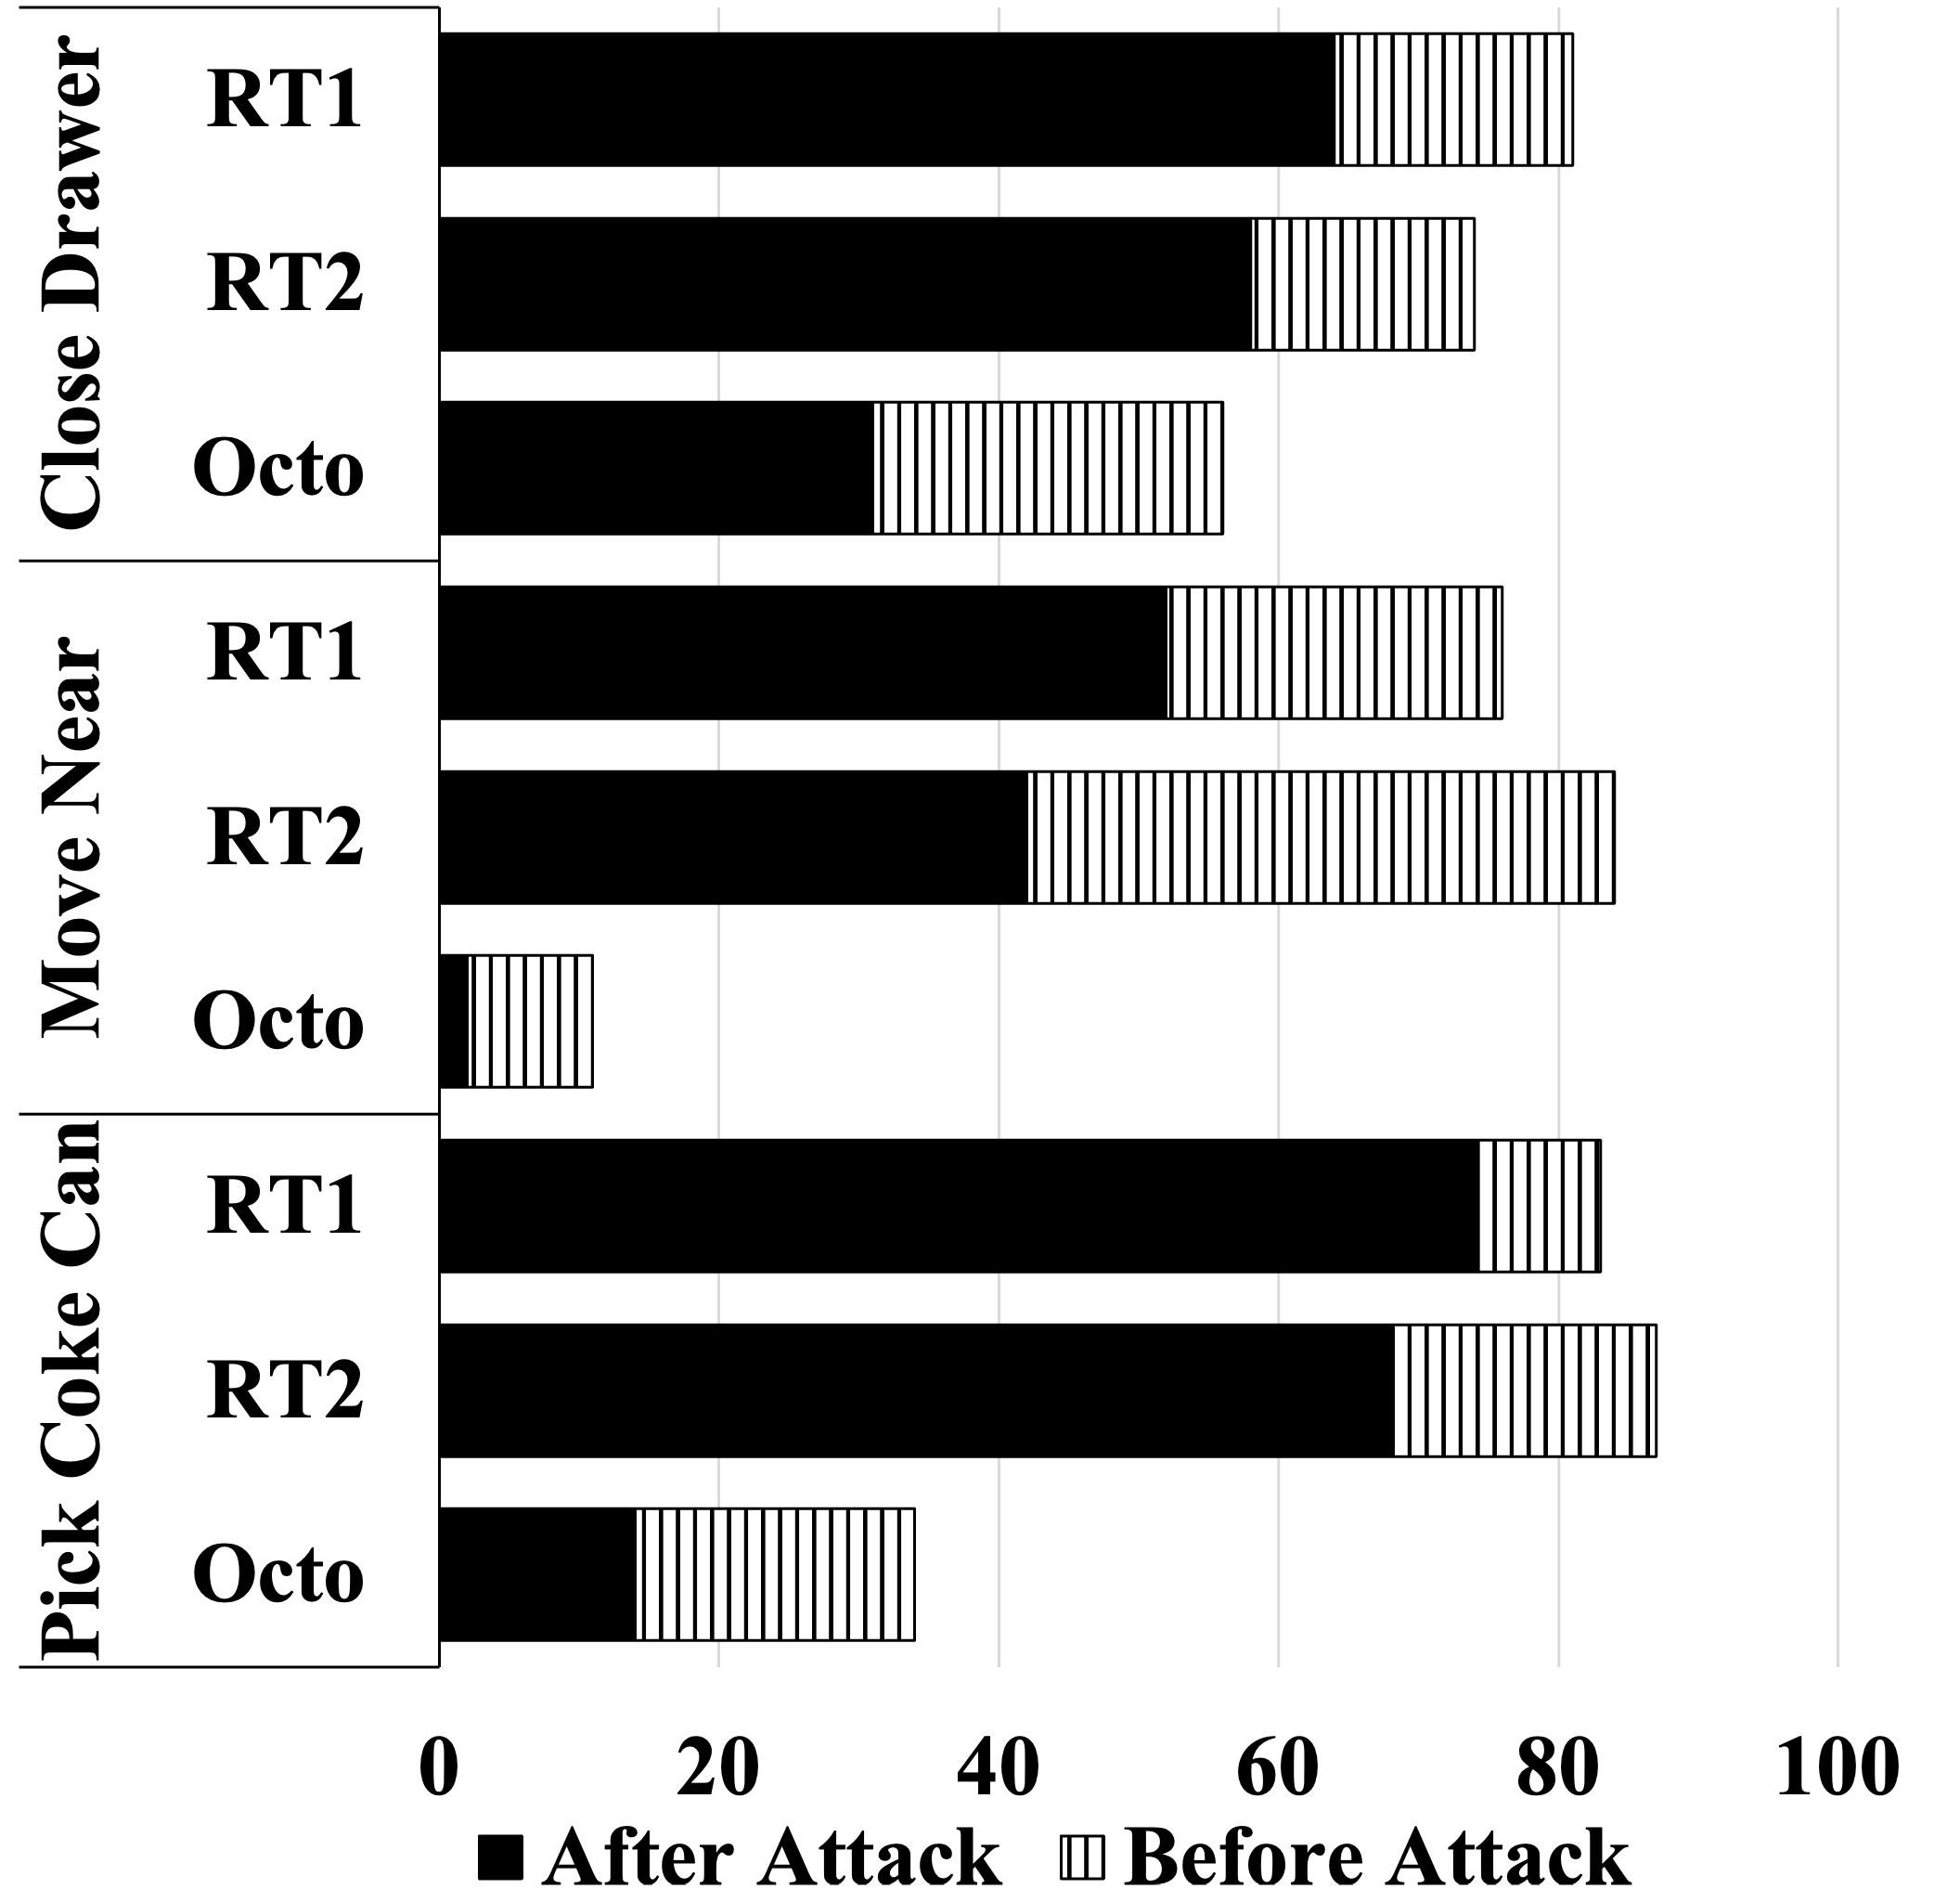
\includegraphics[width=0.9\textwidth]{figures/results/lang_white_box.pdf}\vspace{-2ex}
\caption{Task success rate of models before and after black-box token-based language perturbations.}
  \label{fig:visual_black_box}
\end{minipage}
\vspace{-5ex}
\end{wrapfigure}
 in~\autoref{fig:visual_black_box}, where we observe that the success rate of the models drops significantly after the attack, indicating that even simple token-based perturbations can disrupt the model's performance.
These results demonstrate the potential vulnerabilities of robotic models to adversarial attacks.
In these preliminary experiments we operationalized attack success as a 30\% action-token deviation proxy. In the full evaluation protocol described below, we replace this proxy with task success rate (TSR) under attack as the primary metric and retain action deviation only as a secondary physical-consequence proxy, for which we provide empirical justification through its mapping to end-effector displacement.























\subsubsection{T1-1: White-box Attacks}

White-box attacks exploit full access to the model's architecture, parameters, and gradients.
White-box attacks provide deep insights into model vulnerabilities, enabling precise identification and mitigation of weaknesses. This understanding improves the robustness and security of models, ensuring reliable and safe performance in real-world applications.
While the literature is rich in methods for white-box attacks against various models, the closest model families to generalist robot foundation models are VLMs.
Most evasion attacks against VLM \cite{schlarmann2023adversarial, bailey2023image,gao2024adversarial,wang2024stop,tan2024wolf} typically use gradient-based approaches, \eg PGD~\cite{madry2017towards}, FGSM~\cite{goodfellow2014explaining}, and CW \cite{carlini2017towards}, to generate/optimize perturbation for adversarial samples.
Recent work has begun to move beyond static, single-frame formulations toward trajectory-level redirection and architecture-specific attacks tailored to flow-matching robot policies, which we will build on and compare against~\cite{puthumanaillam2026trajectory,tae2026drift}.
As shown in \autoref{table:attacks_models}, gradient-based attacks can be performed in both the training and inference stages. During training, such attacks manipulate the model's learning process, leading to vulnerabilities such as various poisoning attacks, including recent objective-decoupled backdoor formulations tailored to VLA policies that we will study~\cite{zhou2025badvla}. At the inference stage, they generate adversarial examples by exploiting the model's gradients to deceive the model into making incorrect predictions. 
% \textit{Targeted} attacks seek to drive the model to produce a specific result or action, whereas \textit{untargeted} attacks focus on reducing the overall accuracy of the output.
A recent study \cite{fu2023misusing} shows that seemingly harmless images with trojan-like characteristics can manipulate VLMs to call attacker-specific  third-party tools or external APIs. 
In a different study~\cite{cui2023robustness}, manipulating visual contents that are different from the VLM-specific domain is less effective in deceiving the model. 
%The authorsproposed a context-augmented image classification scheme that demonstrates a significant increase. 
Gao \textit{et al.} \cite{gao2024inducing} introduce verbose images, creating imperceptible perturbations to make VLMs generate longer output sentences. Such an attack raises energy consumption and latency, which can have serious consequences in robotics.
In a cross-modal analysis, creating and refining visual perturbations using adaptive prompts can identify numerous prompts that are effective with specific visual perturbations, resulting in high transferability of adversarial samples \cite{luo2024image}.
% Wu \textit{et al.} \cite{wu2024adversarial} leverage adversarial text sequences to direct gradient-based perturbations on a single trigger image for attacking VLMs.
\ul{In this sub-task, we will propose new attack, Action-Bin Boundary Perturbation (ABBP), and investigate the cross-modal behavior and impact of various evasion and poisoning attacks on robotics models.}

\BfPara{Proposed Attack: ABBP} We propose ABBP, a gradient-based white-box attack designed to exploit the uniform 256-bin discretization of the VLA action space. Because adjacent bins encode physically close but discretely different control signals, ABBP optimizes perturbations to drive predicted action tokens across bin boundaries in a coordinated fashion across all degrees of freedom, subject to a kinematically-consistent Jacobian constraint so the induced action remains reachable. We treat PGD~\cite{madry2017towards}, FGSM~\cite{goodfellow2014explaining}, and C\&W~\cite{carlini2017towards} as baselines rather than contributions. The claimed perturbation-budget advantage over these baselines is not assumed: our formal analysis will compare the required $L_\infty$ budget after normalizing to physical consequence, since a one-bin action shift and a language-token substitution are not directly comparable units. We frame ABBP as research to be conducted, gated by a formal go/no-go check on whether action-space discretization yields a structurally distinct vulnerability.

\subsubsection{T1-2: Gray-box Attacks}
Gray-box attacks exploit partial knowledge of the model, such as its architecture or some aspects of the training pipeline/data. Gray-box attacks provide insights into model vulnerabilities, helping identify and mitigate weaknesses with moderate/limited adversarial knowledge. Multiple evasion and privacy attacks can be conducted under the gray-box scenario (see \autoref{table:attacks_models}).
Existing gray-box attacks often use other vision/language encoders or generative models as surrogates to create adversarial examples, which are transferred to attack VLMs by matching features/embeddings of different encoders to produce adversarial semantics or conceal target noises in the features/embeddings domain for better imperceptibility.
In a study by Zhao \etal \cite{zhao2024evaluating}, pre-trained CLIP \cite{radford2019language} and BLIP \cite{li2022blip} models were used as surrogate models to align adversarial perturbation with textual/image embeddings and generate transferable adversarial examples.
A recent study\cite{wang2024transferable} showed that both modality consistency and discrepancy features can help guiding highly transferable attacks through attention-directed feature perturbation to disrupt modality-consistency features in critical attention regions.
% To assess the adversarial robustness of existing VLMs in out-of-distribution scenarios, Tu \etal \cite{tu2023many} targeted the CLIP~\cite{radford2019language} image-text mismatch to mislead VLMs to produce unrelated visual responses.
In a different work~\cite{wu2024adversarial}, CLIP~\cite{radford2019language} was used as a surrogate to generate attacks against GPT-4o, Gemimi, and Claude agents that embed smaller images within larger images to generate adversarial examples. 
% Wang \etal \cite{wang2023instructta} employ a text-to-image generative model to invert the target response into a corresponding image, using the same surrogate visual encoder as the victim VLM to extract instruction-aware features from both the adversarial image and the target image. In addition, they improve transferability by using paraphrased instructions generated from an LLM.
\ul{In this sub-task, we will explore various gray-box evasion ({\eg} prompt injection and jailbreak) and privacy ({\eg} membership and attribute inference) attacks against robotics models.} Language-modality attacks ({\eg} prompt injection and jailbreak) apply only to language-conditioned models ({\eg} RT-2, OpenVLA, and Octo) and exclude vision-only models such as ACT.

\subsubsection{T1-3: Black-box Attacks}
Black-box attacks operate without any access to the model's architecture, parameters, or gradients. These attacks rely on input-output pairs to infer vulnerabilities, making it possible to identify and exploit weaknesses despite limited information about the system. 
Given their more plausible and real-world-applicable threat assumptions and adversarial capabilities, black-box attacks are challenging and critical to understanding how models can be compromised in real-world applications. 
Although numerous studies have explored and proposed various methods for such attacks on vision models~\cite{guo2019simple,hallyburton2022security,abdukhamidov2022black, juraev2024attack,abdukhamidov2023microbial} and LLMs~\cite{li2023deepinception,yao2024fuzzllm,ding-etal-2024-wolf,wei2023jailbreak,deng2024pandora}, there is limited research on these threats to VLMs~\cite{zhang2024avibench,dong2023robust} and only nascent, isolated studies targeting robotic foundation models, such as jailbreaking and backdoor attacks~\cite{badvla,advvla}, motivating the systematic study we propose here.
The lesson learned from black-box attacks against LLMs is that even with the advanced safety alignment techniques in commercial LLMs, attackers still create sophisticated methods that bypass model defenses against harmful content. 
% The incorporation of vision models and LLMs into robotic learning is receiving more attention~\cite{rt-1,rt-2,bousmalis2023robocat}, which makes it crucial to study whether inherited vulnerabilities can impact the end-to-end robotic model.
% Tan \textit{et al.} \cite{tan2024wolf} explore the indirect propagation of malicious content by subtly influencing a single 'wolf' agent to compel other 'sheep' agents in the society to produce malicious content.
% They find that this form of threat can be achieved through the indirect nature of manipulation on the input, without requiring in-depth access to the model's parameters.
A recent study~\cite{zhang2024avibench} showed that VLMs can be vulnerable to decision-based black-box visual instructions.
Moreover, Dong \etal~\cite{dong2023robust} shows that transfer-based attacks can succeed against well-defended VLMs.
Recent work has begun to construct universal, transferable adversarial patches that carry across robot policies in physical settings, which we will build on and compare against~\cite{lu2026whenrobots}.
% Wang \textit{et al.} \cite{wang2024stop} evaluate the adversarial robustness of MLLMs employing chain of thought (CoT) reasoning, finding that models using CoT generally exhibit significantly higher robustness under both answer and rationale attacks compared to models without CoT.
% Based on these findings, they introduce a novel stop-reasoning attack technique that effectively circumvents the robustness enhancements induced by CoT.
% Guo \textit{et al.} \cite{guo2024efficiently} utilize diffusion models to generate natural, unrestricted adversarial examples.
% They employ Adaptive Ensemble Gradient Estimation to ensure the adversarial examples produced contain natural adversarial semantics, thus enhancing their transferability.
% Furthermore, they use the GradCAM-guided Mask method to disperse adversarial semantics throughout the image, rather than concentrating them in a specific area, thereby improving the quality of the adversarial examples.
% Dong \textit{et al.} \cite{dong2023robust} investigate the adversarial robustness of Google's Bard as a representative of VLMs through transfer-based attacks, demonstrating that these adversarial images are highly transferable and effective at deceiving other VLMs.
% Additionally, they identify two of Bard’s defense mechanisms—face detection and toxicity detection in images—and successfully target these features in their attacks.
\ul{In this sub-task, we will explore various black-box evasion and privacy ({\eg} data reconstruction and prompt stealing) attacks against robotic models.} Language-based attacks such as prompt stealing apply only to language-conditioned models and exclude vision-only models such as ACT.

\BfPara{Proposed Attack: Temporal Trajectory Drift Attack (TTDA)} We propose TTDA, a trajectory-level gray- and black-box attack targeting the multi-step action chunk predicted by chunking policies such as Octo~\cite{team2024octo}. TTDA crafts slowly-accumulating perturbations so each individual step satisfies per-step kinematic limits and evades naive per-step anomaly checks, while the cumulative trajectory drifts toward a task-failing or workspace-violating end configuration. This attack surface is structurally absent in single-output VLMs. We will formalize sufficient conditions for such drift and characterize how chunk length affects feasibility. We will extend TTDA to flow-matching policies ({\eg} pi-0~\cite{black2024pi_0}), where the denoising trajectory provides an analogous sequence structure, as a scale-up objective in Years~3 and~4 contingent on model availability.

\subsubsection{T1-4: Defense Strategies}



 Several existing defenses (shown in~\autoref{tab:defense}) designed originally for VLMs will be examined against robotic models.
These defenses can be applied in the inference and training stages of the model development.
Inference-based defenses include anonymous detection~\cite{zhang2023mutation,gou2024eyes,pi2024mllm} and prompt engineering~\cite{wu2023jailbreaking,wang2024adashield,chen2023can} methods.% that design and optimize the prompt to enhance the defense mechanism of the model. 
JailGuard \cite{zhang2023mutation} and ECSO \cite{gou2024eyes} are designed to identify multimodal jailbreaking attacks during inference.
MLLM-Protector~\cite{pi2024mllm} proposes an inference-time detection of harmful inputs and correct (detoxify) the output responses. InferAligner~\cite{wang2024inferaligner} proposes an inference time safety alignment method for VLM. 
Alignment methods align model behaviors with expected values and intentions. The main techniques are Instruction Tuning and Reinforcement Learning from Human Feedback.
Regarding training-time VLM defenses, most work \cite{chen2023dress,zhang2023adversarial,li2024one} constructs robust natural language feedback or robust text prompts in VLM to defend against potential attacks, while \cite{li2024red,yang2024robust} proposes to train robust VLM by further fine-tuning or contrastive learning.
Recent work has begun to develop VLA-specific defenses, including structure-aware robust fine-tuning, randomized smoothing for certified robustness, and backdoor token reconstruction, which we will build on and compare against~\cite{zhang2026structure,seferis2025randomized,li2026whenattention}.
{\ul{In this sub-task, we will develop and explore the effect of various defenses against attacks on robotic models.}}
% {\vspace{-1ex}}


\BfPara{Action-Space Anomaly Detection} Beyond porting inference- and training-time VLM defenses, we propose 
a robotics-specific defense unavailable to general VLMs: an action-space anomaly detector operating on predicted actions rather than inputs. The detector flags out-of-distribution and kinematically-implausible actions, such as predictions violating the reachable workspace, joint limits, or defined safety zones, independent of the input modality under attack. Because the detector inspects the action output directly, this defense complements input-side defenses and remains effective when the compromised modality is unknown. We will characterize the detection rate and false-positive trade-off across embodiments and attack types.


\BfPara{Proposed Defenses: TACD and AGAT} We instantiate the action-space defense as the Temporal Action Consistency Detector (TACD), which raises detection from the per-step level to the sequence level to catch TTDA-style drift that per-step kinematic checks miss by construction. TACD uses a single multi-task trajectory-forecasting model conditioned on a task embedding, trained jointly on the benign demonstrations of all tasks to avoid per-task model proliferation, with a per-task threshold calibrated on held-out benign episodes. We complement detection with Action-Grounded Adversarial Fine-Tuning (AGAT), which augments fine-tuning with kinematically-constrained ABBP-style perturbations. To remain compute-feasible on the available hardware, AGAT is implemented with LoRA rank-16 adaptation (roughly 25M trainable parameters) rather than full-model backpropagation. We will evaluate TACD and AGAT against at least three baseline defenses (input smoothing, VLM-ported adversarial training, and ensemble voting), reporting detection-rate versus false-positive Pareto curves per embodiment and attack type.

\subsubsection{Evaluation Plan and Deliverables}
\begin{wraptable}{r}{0.36\textwidth}{\vspace{-3ex}}
\centering
\caption{(\textbf{T})raining \& (\textbf{I})nference defenses.}\vspace{-2ex}
\label{tab:defense}
\resizebox{\linewidth}{!}{%
\begin{tabular}{l}
\toprule
\cite{zhang2023mutation}  ~\textbf{I}$\rightarrow$  Anonymous detection \\ 
\cite{gou2024eyes}   ~\textbf{I}$\rightarrow$   Anonymous detection \\ 
\cite{pi2024mllm} ~\textbf{I}$\rightarrow$   Anonymous detection \\ 
\cite{wu2023jailbreaking}   ~\textbf{I}$\rightarrow$   Prompt engineering \\
\cite{wang2024adashield}   ~\textbf{I}$\rightarrow$   Prompt engineering \\ 
\cite{chen2023can}   ~\textbf{I}$\rightarrow$   Prompt engineering \\
\cite{wang2024inferaligner}   ~\textbf{I}$\rightarrow$   Alignment process \\
\cite{zhang2023adversarial}  ~\textbf{T}$\rightarrow$  Robust  feedback/prompt \\
\cite{chen2023dress}  ~\textbf{T}$\rightarrow$  Robust feedback/prompt \\
\cite{li2024one}  ~\textbf{T}$\rightarrow$  Robust  feedback/prompt \\
\cite{yang2024robust}  ~\textbf{T}$\rightarrow$  Fine-tuning/Contrastive learning \\
\cite{li2024red}  ~\textbf{T}$\rightarrow$  Fine-tuning/Contrastive learning \\
 \bottomrule
\end{tabular}
}\vspace{-2ex}
\end{wraptable}
We will benchmark various attacks (\autoref{table:attacks_models}) and defenses (\autoref{tab:defense}) against state-of-the-art robotic models using comprehensive datasets. Our primary metric is task success rate (TSR) under attack, a binary task-completion judgment using the two-point scoring system of our preliminary experiments. We retain the 30\% action-token deviation as a secondary physical-consequence proxy, alongside Attack Success Rate, \textit{Contain} \cite{lu2024test} (presence of attacker-specific action tokens), \textit{Exactmatch} \cite{luo2024image,lu2024test} (perfect match with attacker-specific tokens), transferability, and perturbation imperceptibility. 
To further ground these token-level metrics in physical consequences, we report maximum end-effector action displacement and the rate of safety-zone and force-threshold violations. We evaluate our proposed defenses against at least three baseline defenses, and we construct a full model~$\times$~model~$\times$~attack transferability matrix across the model families and embodiments in our scope. We report all metrics as mean~$\pm$~std over at least ten runs with multiple seeds, and assess significance with Welch's $t$-test.
We will align this protocol with recent physically-grounded evaluation practice for robot policies~\cite{sun2026maniparena}.
Deliverables include: \cib{1} a comprehensive framework of attack vectors (and defenses) specific to robotic models
with target modalities, tasks, and embodiments, \cib{2} open-source implementation includes datasets, developed attacks, defenses, and evaluations, and \cib{3} academic publications/reports/labs on findings and methodologies.




\subsection{T2: Modality-inherited Vulnerabilities and Impact on Multimodal Robots}
This task aims to examine the security and defense strategies derived from the targeting of one or more modalities used by robots. 
Although much progress has been made in designing adversarial attacks in individual modalities (\eg vision or language), the interaction between modalities remains less explored. Existing attackers, even with multimodal systems, generally treat the perturbations of different modalities separately and design them independently. 
However, this results in less interactive relations between the perturbed multimodal inputs and can be easily recognized by security alignment methods (\ie methods
to align the model behavior with expected values and intentions). 
In addition, along with visual and textual instructions, other modalities can be incorporated in the training of generalist robots. Some of these modalities can be sensory information, tabular environment data, or supplementary interpretation maps (\ie maps that indicate the region of importance in recent outputs). 

\subsubsection{Multimodal Adversarial Attacks}
To date, emerging foundation models in robotics focus mainly on visual and textual instruction. With the current trend of democratization of data and models, we expect and plan to explore more modalities as they emerge as common information used by robots.
We note that incorporating additional modalities into the system provides attackers with more physical avenues to launch attacks.
\ul{Our aim is to explore novel ways to reveal vulnerabilities by crafting ``\textit{tightly-multimodal}'' adversarial examples that simultaneously perturb visual and textual input with strong connections.} 
We will target the vision-language coupling mechanism specific to each model, namely FiLM in RT-1~\cite{rt-1}, a projection MLP in OpenVLA~\cite{kim2024openvla}, and cross-attention in Octo~\cite{team2024octo}, and formulate a model-specific co-perturbation objective at each mechanism so the visual and textual perturbations co-reinforce at the grounding layer. To test coupling on a further language-conditioned policy, we include OpenVLA-OFT or a language-conditioned Octo variant, and we exclude vision-only policies such as ACT from this multimodal scope. We present T2 as a scale-up track in Years~3 and~4 that builds on the attack baselines established in T1.
This includes studying the interactions and dependencies between modalities to create more effective cross-modal attacks that can evade current defenses. For example, Multi-key strategies~\cite{walmer2022dual} could be used to improve the connections between multimodal perturbations and co-control the attack.
Multimodal prompt injection attacks simultaneously alter both textual and visual modalities, injecting adversarial semantics into multiple modalities to enhance the possibility of overcoming alignment methods.
Recent studies \cite{qi2024visual,shayegani2023jailbreak} show that adversarial perturbations of visual and textual modalities can jointly succeed in creating malicious injections.
Recent work has begun to explore physical attention-hijacking and patch attacks that target the vision-language grounding of robot policies, which we will build on and compare against~\cite{zhang2026structure,yin2026vlaguard}.
By understanding and leveraging these interactions, we aim to develop more robust defense mechanisms that can protect against sophisticated multimodal adversarial attacks. We will also assess robustness techniques such as CleanCLIP~\cite{bansal2023cleanclip}, which retrains multimodal representations to reduce cross-modal misalignment, as a complementary defense against these attacks.
%Besides, Chen \textit{et al.} \cite{chen2023can} proposes a multimodal benchmark designed to protect specific categories of personal information in a simulated scenario. In their work, they construct textual and visual prompt injection attacks through adversarial prefixes and by rendering misinformed text onto the image, thereby inducing the model to disclose protected personal information.
\ul{In this task, variations of attacks by}~{\cite{qi2024visual,walmer2022dual}} \ul{will be implemented against robotic models.}



\subsubsection{Evaluation Plan and Deliverables}

We will benchmark various multimodal attacks, measuring their effectiveness across multiple robot embodiments and tasks. As in T1, our primary metric is task success rate (TSR) under attack, with the 30\% action-token deviation retained as a secondary proxy.
In addition to attack evaluation metrics, such as Attack Success Rate, 
\textit{Contain} \cite{lu2024test}, \textit{Exactmatch} \cite{luo2024image,lu2024test}, transferability, and imperceptibility, we will use cross-modal benign-adversarial shifting to evaluate the impact of different modality in achieving adversarial objective.
For example, assess whether the attack can succeed or change behavior when an input to a successful multimodal attack (\ie $\mathcal{M}(\mathcal{P}(\bm{x},\bm{t}_{in}))\rightarrow\bm{a}_{out}'$) is mutated, \eg $\{\mathcal{P}(\bm{x},\bm{t}_{in})\} \rightarrow\{\mathcal{P}(\bm{x}),\bm{t}_{in}\}$ or $\{\bm{x},\mathcal{P}(\bm{t}_{in})\}$.
The mutation process can be adjusted to alter the extent of shifts required to facilitate behavior change.
As in T1, we also report maximum end-effector action displacement and safety-zone and force-threshold violation rate, each as mean~$\pm$~std over at least ten runs with significance assessed by Welch's $t$-test, and we contribute the multimodal attacks to the full cross-model transferability matrix.
We will align this protocol with recent physically-grounded evaluation practice for robot policies~\cite{sun2026maniparena}.
Deliverables include: \cib{1} a comprehensive framework for multimodal attacks/defenses against robotic foundation models, analyzing how vulnerabilities propagate across modalities, \cib{2} open-source implementations of developed multimodal attacks, defenses, and benchmarks, and \cib{3} academic publications/reports/labs on findings and methodologies.

 


\subsection{T3: Benchmarks Toward Safe and Trustworthy Robotic Models}
This task aims to examine the safety and interpretability of robotic foundation models, develop methods to improve the robustness, safety, and interpretability of the models.
The importance of trustworthiness in robotic models cannot be overstated, particularly as large foundation models in robotics continue to emerge and possibly integrate in multiple downstream tasks within various sectors. 
Ensuring the safety of these robotic systems is paramount, as any malfunction or unexpected behavior can cause significant harm or damage in environments where robots operate alongside humans. 
Transparency is another challenge for these models and systems.
Generally, transparency (\ie explainability or interpretability) poses a major challenge in large multimodal models, given that intricate models and the combination of various input types can produce actions that are not easily understood.
% This lack of transparency can obscure potential biases embedded within algorithms/data, leading to unfair or discriminatory outcomes. 
Solving these challenges requires rigorous testing benchmarks and protocols to ensure that robotic models perform reliably, safely, and uphold ethical integrity.



\subsubsection{T3-1: Safety in Robotic Models}
Ensuring safety has been a crucial aspect of robotics since the introduction of the earliest industrial robots.
Safety, defined as the condition of being protected from or unlikely to cause danger, risk, or injury, is a critical issue in Industrial Robotics, where more than 1.5 million industrial robots operate in factories worldwide.
Although there are high standards of operational safety of robotics, such as ISO 13482:2014 personal care robots, ISO 10218-1 and ISO 10218-2 for industrial robots, and ISO/TS 15066 for collaborative robots, safety in foundation robotic models should address possible harm or bias in output given certain inputs (benign or adversarial).
In relation to such safety aspects, there have been no previous works that addressed such issues, except physical safety~\cite{FoschVillaronga2015CreationOA,RePEc:eps:cepswp:26204,10.3389/frobt.2022.1002226}.
A study by~\cite{fosch21} explores the interaction between robots, cybersecurity, and safety from a European legal perspective, illustrating cybersecurity challenges and their subsequent safety implications with the concrete example of care robots.
Another study by~\cite{tadokoro19} provides an overview of the ImPACT Tough Robotics Challenge and Strategy for Disruptive Innovation in Safety and Security (ImPACT-TRC), a project by the Japan Cabinet Office focusing on robotic technologies for disaster response, recovery, and preparedness.
To ensure the safety of the robot model, an effective and innovative validation process is crucial. This is difficult due to the restricted number of validation scenarios which may fail to reflect real-world intricacies, along with the significant computational expense of identifying infrequent failures.
Several prior studies have established standardized push-recovery testbeds by imposing consistent external perturbations on the legged robot under varying control strategies \cite{zhangei2023quadruped-tro, weng2023standard-legged-test, weng2023comparability}.
Recent work has begun to release dedicated VLA security benchmarks and physically-grounded evaluation suites, which we will build on and compare against~\cite{li2025attackvla,sun2026maniparena}.

\ul{To evaluate the safety measures of generalist robot models, we propose examining various defense mechanisms that enhance robustness and safety. We will develop methods similar to JailGuard~}\cite{zhang2023mutation}\ul{, ECSO~}\cite{gou2024eyes}\ul{,  MLLM-Protector~}\cite{pi2024mllm}\ul{, InferAligner~}\cite{wang2024inferaligner}\ul{ to detect/normalize safety-critical outputs during inference.}


\subsubsection{T3-2: Interpretation of Robotic Models}

Regardless of the architecture or domain, it is essential that we can interpret and explain the decisions made by the AI model.
Methods for interpretability can be categorized into gradient- and inference-based methods. 
Gradient-based methods typically leverage inter- and intra-modality interactions to provide visual explanations for the decisions, whereas inference-based methods are designed to provide explanations to specific aspects or components of the models and may be limited to particular tasks.




\BfPara{Gradient-based Interpretation Methods} 
Robotic models are mostly incorporate transformer-based components, which can use
attention maps for interpretation. 
Variants of these methods have been discussed in the literature, such as the Attention Rollout \cite{abnar2020quantifying}, which integrates layers to produce an average attention map. %The work by~\cite{voita-etal-2019-analyzing} specifically adapted the LRP method for transformers, addressing computational challenges.
A recent study \cite{DBLP:journals/corr/abs-2106-12620} proposes $\text{IA-RED}^2$, enhancing transformer efficiency with human-understandable architecture.
Other methods include AttCAT~\cite{DBLP:conf/nips/QiangPLLJZ22}, B-cos~\cite{DBLP:journals/corr/abs-2301-08669}, Vision DiffMask~\cite{DBLP:conf/cvpr/NalmpantisPGPA23}, and ICE~\cite{DBLP:conf/cvpr/ChoiJH23}.
In the VLM domain and multimodal interpretation, Relevancy Map \cite{chefer2021generic} uses self-attention and co-attention with classification tokens to produce a relevancy map, tracking interactions across modalities, and back-propagating relevancies. The approach works for unimodal and multimodal models.
VL-InterpreT \cite{aflalo2022vl} serves as a tool providing an interactive interface to examine the interactions among the modalities using a bottom-up approach. It employs four modality attention heads: language-to-vision attention, vision-to-language attention, language-to-language attention, and vision-to-vision attention, enabling the examination of interactions both within and across modalities.
Other methods include MultiViz \cite{liang2022multiviz} and gScoreCAM~\cite{chen2022gscorecam}.
 



\BfPara{Inference-based Interpretation Methods} 
Most interpretation techniques for VLMs rely on inference-based methods, which are designed to investigate specific components of the model, making them difficult to generalize. 
The Vision And Language Understanding Evaluation (VALUE) method described in \cite{cao2020behind} introduces various inference tasks aimed at understanding the impact of pre-training on learned representations.
The research indicates that pre-trained VLMs prioritize language over vision and that some attention heads are responsible for capturing interactions across modalities.
In another study~
\cite{dahlgren-lindstrom-etal-2020-probing}, three inference tasks for visual-semantic space were introduced to capture image-caption relations.
% A study by~\cite{hendricks2021probing} presents inference tasks for verb understanding using image-sentence pairs with 421 verbs from the Conceptual Captions dataset~\cite{sharma2018conceptual}. 
A study by~\cite{DBLP:conf/aaai/SalinFAF22} introduces inference tasks to understand and compare representations by VLMs from pre-trained and finetuned versions. 


%In addition, data sets are designed carefully for multimodal
%probing, trying to reduce dependency on bias while making predictions. While probing tasks are helpful and can answer meaningfully with regard to particular problems, they have to be carefully crafted for relevant results and are very specific. At times, extra models or classifiers are required for probing, making the probing tasks applicable to selected models only.


\ul{We aim to investigate both gradient- and inference-based techniques to better understand predicted robotic actions. We will develop methods to interpret the decisions made by robotic models.}
Recent work has begun to explore spatial-grounding attribution and neuro-symbolic spatial reasoning for embodied models, which we will build on for action-level interpretation~\cite{schofield2026chain,jahangard2025multimodal}.


\subsubsection{Evaluation Plan and Deliverables}
Visualization techniques, \eg heatmaps and saliency maps, will be used to interpret how the model makes decisions under both normal and adversarial conditions.
Case studies on specific instances (\ie instruction-action pairs) where the model fails or succeeds will be conducted to understand the behavior of the model.
There will be human-in-the-loop evaluations that include reviewing and interpreting the results, ensuring that the methods align with human understanding and expectations.
Deliverables include: \cib{1} benchmarks for safety and interpretability of robotic foundation models, \cib{2} open-source implementations of developed safety and interpretability methods, and \cib{3} academic publications/reports/labs on findings and methodologies.


\subsection{Work Plan, Timeline, and Team}

\BfPara{Staged Scope} We stage the program into Phase 1 (Years~1 and~2) and a Phase 2 (Years~3 and~4). Phase 1 targets open and architecturally complementary models on two embodiments (Xarm7 and the Google robot), and develops ABBP and TTDA with ported baselines together with the TACD and AGAT defenses and their baselines. 
The Phase 2 adds emerging models, multimodal analysis, certified-robustness defenses, and the full public release of VLA-SecBench. 
\autoref{fig:workplan_timeline} summarizes the schedule of the research-plan tasks under the calendar aligned to the budget period.

\begin{figure*}[t]
\centering
\resizebox{\textwidth}{!}{%
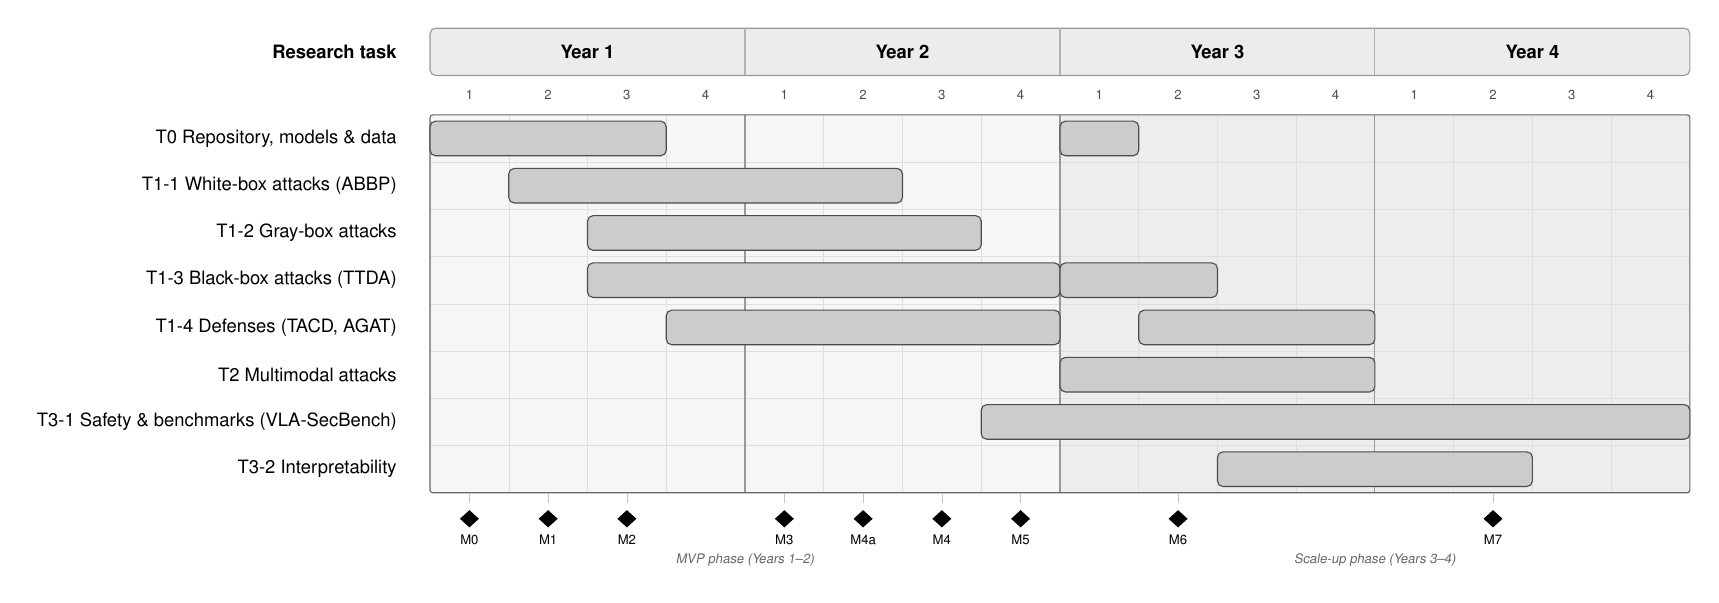
\begin{tikzpicture}[font=\scriptsize\sffamily,
  bar/.style={fill=gray!40, draw=black!70, rounded corners=2pt},
  ]
  %%% phase (MVP / Scale-up) background shading %%%
  \fill[gray!7]  (0,-3.4) rectangle (8,1.4);
  \fill[gray!14] (8,-3.4) rectangle (16,1.4);

  %%% horizontal row separators %%%
  \foreach \hy in {0.80,0.20,-0.40,-1.00,-1.60,-2.20,-2.80}
    \draw[very thin, gray!25] (0,\hy) -- (16,\hy);

  %%% vertical quarter gridlines %%%
  \foreach \gx in {1,2,3,5,6,7,9,10,11,13,14,15}
    \draw[very thin, gray!25] (\gx,-3.4) -- (\gx,1.4);
  %%% year boundary lines %%%
  \foreach \gx in {4,8,12}
    \draw[thin, black!40] (\gx,-3.4) -- (\gx,1.4);
  %%% outer chart border %%%
  \draw[black!60, rounded corners=1pt] (0,-3.4) rectangle (16,1.4);

  %%% year header band %%%
  \fill[gray!15, draw=black!40, rounded corners=2pt] (0,1.9) rectangle (16,2.5);
  \foreach \gx in {4,8,12} \draw[black!30] (\gx,1.9) -- (\gx,2.5);
  \node[font=\scriptsize\bfseries\sffamily] at (2,2.2)  {Year 1};
  \node[font=\scriptsize\bfseries\sffamily] at (6,2.2)  {Year 2};
  \node[font=\scriptsize\bfseries\sffamily] at (10,2.2) {Year 3};
  \node[font=\scriptsize\bfseries\sffamily] at (14,2.2) {Year 4};

  %%% quarter tick numbers %%%
  \foreach \g in {1,...,16} {
    \pgfmathtruncatemacro{\qn}{mod(\g-1,4)+1}
    \node[font=\tiny\sffamily, text=black!70] at (\g-0.5,1.65) {\qn};
  }

  %%% left-hand labels %%%
  \node[anchor=east, font=\scriptsize\bfseries\sffamily] at (-0.3,2.2)  {Research task};
  \node[anchor=east] at (-0.3,1.10)  {T0 Repository, models \& data};
  \node[anchor=east] at (-0.3,0.50)  {T1-1 White-box attacks (ABBP)};
  \node[anchor=east] at (-0.3,-0.10) {T1-2 Gray-box attacks};
  \node[anchor=east] at (-0.3,-0.70) {T1-3 Black-box attacks (TTDA)};
  \node[anchor=east] at (-0.3,-1.30) {T1-4 Defenses (TACD, AGAT)};
  \node[anchor=east] at (-0.3,-1.90) {T2 Multimodal attacks};
  \node[anchor=east] at (-0.3,-2.50) {T3-1 Safety \& benchmarks (VLA-SecBench)};
  \node[anchor=east] at (-0.3,-3.10) {T3-2 Interpretability};

  %%% research-task bars (active quarters) %%%
  \fill[bar] (0,0.88)   rectangle (3,1.32);   % T0
  \fill[bar] (8,0.88)   rectangle (9,1.32);   % T0 (refresh)
  \fill[bar] (1,0.28)   rectangle (6,0.72);   % T1-1
  \fill[bar] (2,-0.32)  rectangle (7,0.12);   % T1-2
  \fill[bar] (2,-0.92)  rectangle (8,-0.48);  % T1-3
  \fill[bar] (8,-0.92)  rectangle (10,-0.48); % T1-3 (extend)
  \fill[bar] (3,-1.52)  rectangle (8,-1.08);  % T1-4
  \fill[bar] (9,-1.52)  rectangle (12,-1.08); % T1-4 (certified)
  \fill[bar] (8,-2.12)  rectangle (12,-1.68); % T2
  \fill[bar] (7,-2.72)  rectangle (16,-2.28); % T3-1
  \fill[bar] (10,-3.32) rectangle (14,-2.88); % T3-2

  %%% milestone diamonds along the bottom axis %%%
  \foreach \mx/\ml in {0.5/M0, 1.5/M1, 2.5/M2, 4.5/M3, 5.5/M4a, 6.5/M4, 7.5/M5, 9.5/M6, 13.5/M7} {
    \draw[very thin, gray!45] (\mx,-3.4) -- (\mx,-3.53);
    \fill[black, draw=black] (\mx,-3.63) -- (\mx-0.11,-3.73) -- (\mx,-3.83) -- (\mx+0.11,-3.73) -- cycle;
    \node[font=\tiny\sffamily, anchor=north, inner sep=1pt] at (\mx,-3.9) {\ml};
  }

  %%% phase captions %%%
  \node[font=\tiny\itshape\sffamily, text=black!60] at (4,-4.25)  {MVP phase (Years 1--2)};
  \node[font=\tiny\itshape\sffamily, text=black!60] at (12,-4.25) {Scale-up phase (Years 3--4)};
\end{tikzpicture}%
}
\caption{Gantt-style work-plan timeline. Calendar aligned to the anticipated award start (May~2027): Year~1 = May~2027--Apr~2028, \ldots, Year~4 = May~2030--Apr~2031; quarters Q1~(May--Jul), Q2~(Aug--Oct), Q3~(Nov--Jan), Q4~(Feb--Apr). Bars indicate active quarters; diamonds mark milestones (M0--M7). {\footnotesize\textbf{Milestones:} \textbf{M0} compute/NSF ACCESS allocation secured; \textbf{M1} ABBP formal specification; \textbf{M2} MVP model zoo operational; \textbf{M3} ABBP vs.\ PGD comparison; \textbf{M4a} preliminary TACD false-positive check; \textbf{M4} formal TACD detection gate; \textbf{M5} VLA-SecBench v0.5 \& pi-0 availability; \textbf{M6} multimodal coupling benefit shown; \textbf{M7} VLA-SecBench v1.0 release.}}
\label{fig:workplan_timeline}
\end{figure*}




% \subsection{Task Implementation and Timeline}

% \begin{figure*}[h]
%   \centering\vspace{-2ex}
%   \includegraphics[width=0.63\textwidth]{figures/grant1_1.pdf}\vspace{-2ex}
%   \caption{Proposed work plan and timeline.}
%   \label{fig:timeline}
% \end{figure*}

\section{Broader Impacts of the Proposed Work} \label{sec:broader_impacts}

Generalist robot foundation models are increasingly being deployed in safety-critical environments, \eg manufacturing, logistics, healthcare, and public service. Adversarial vulnerabilities in robotic policies appear as physical displacements, velocity anomalies, and force-threshold violations. The broader impacts of this project address scientific, operational, societal, and workforce dimensions:
\cib{1} \textbf{Cross-disciplinary scientific impact:} 
This research bridges adversarial machine learning, computer vision, and cyber-physical control theory. By shifting evaluation from image-space to physical consequence metrics (task success degradation, trajectory deviation, and joint-limit violations), this work provides a foundation for evaluating embodied models. Analyzing coupling layers in multimodal models provides the broader multimodal AI community with foundational insights into cross-modal error propagation. 
\cib{2} \textbf{Open-source resources via VLA-SecBench:} 
To promote open science and reproducibility, all attack, defense, and evaluation benchmarks developed in this project, including {VLA-SecBench}, will be published under open-source licenses. This guarantees full methodological transparency and provides the research community with standardized, evaluation protocols to benchmark emerging robot foundation models across diverse embodiments.
This contributes toward enabling their safe deployment in critical systems, increasing public acceptance and trust in robotic systems, and fostering a security-conscious generation of researchers and practitioners in the field of robotics and AI.
\cib{4} \textbf{Workforce development:} 
The project directly interfaces with Loyola University Chicago's NSF CyberRamblers Scholarship for Service (SFS) program, for which the PI serves as co-PI. CyberRamblers scholars will participate directly in research tasks, gaining hands-on experience in robotic security, embodied AI, and physical system defense. Additionally, undergraduate researchers will be integrated into the research program through the Loyola Undergraduate Research Opportunities Program (LUROP) and competitive university fellowships (Mulcahy, Carbon, and Provost).
\section{Results From Prior NSF Support}

\BfPara{Award \# 2335700: Education DCL: EAGER: Developing Experiential Cybersecurity and Privacy Training for AI Practitioners} (PI: Abuhamad, 11/01/2023 -- 10/31/2025, \$299,905.00). 
\textbf{Intellectual Merit:} The project establishes experiential cybersecurity training for AI professionals. The goal
is to raise AI workers' awareness of security and privacy risks by developing and evaluating a comprehensive 12-workshop experiential training program. The workshop series provides the knowledge and skills needed to build AI systems that are not only technically sound from an AI perspective, but also secure, ethical, and privacy-preserving. 
\textbf{Broader Impacts:}
The completion of the program will result in a workforce proficient in the use of AI with an understanding of its cybersecurity issues. The program's materials and outcomes will be shared through various channels to promote responsible AI practices. Educational resources, case studies, and research papers will be available on a dedicated website. %Findings will also be published in reputable conferences and journals.




\BfPara{Award \# 2336386: CyberCorps Scholarship for Service: CyberRamblers Bolster National Security} (Co-PI: Abuhamad, 01/01/2024 --  12/31/2028, \$3,803,006.00). 
\textbf{Intellectual Merit:}
The CyberRamblers program enhances the interdisciplinary activities of the Loyola Center for Cybersecurity. Scholars in this program engage in interdisciplinary research and education, which fosters critical thinking, independence, teamwork, and technical knowledge essential for a cybersecurity career. The B.S. in Cybersecurity curriculum emphasizes a hands-on approach to learning, enabling students to apply concepts and confidently utilize the latest tools.
\textbf{Broader Impacts:}
Twenty undergraduate students will be trained through a program aimed at preparing them for careers in cybersecurity, addressing the high demand for professionals in this field. The program's goal includes having 50\% of participants from underrepresented groups. This initiative will benefit society by enhancing national security and protecting various critical sectors such as energy, commerce, finance, education, healthcare, manufacturing, and agriculture against cyber-attacks.


%\section{Education and Outreach Plan}
Our Education and Outreach Plan aims to reach Chicago audiences, including K-12 students and educators, undergraduate and graduate students, and practitioners in the field of robotics and cybersecurity. 
The main goals are to offer educational resources, engage diverse communities, and inspire future careers in robotics, cybersecurity, and related fields.
% Educational robots can significantly enhance learning experiences by promoting active engagement, problem-solving, and collaboration among students. 
As part of our support for Chicago communities, the PI will focus on leveraging the unique opportunities and resources available in Chicago and Loyola University.   
% Since the PI is a faculty of Loyola University Chicago, the PI will develop robotics classes and provide guest lectures, and seminars. This will include several key initiatives:

\BfPara{Robotic Security Course Development} 
Loyola University Chicago has been designated as a Center of Academic Excellence (CAE) in Cyber Defense by the NSA/DHS in June 2020 and offers robust cybersecurity and computer science programs.
PI is an active member of the center and CAE community and will leverage these resources to design and develop a comprehensive robotic security course for university-level students. 
This course will cover a variety of topics, including basic robotics principles, programming, mechanical design and embodiments, AI integration, and emerging threats and countermeasures in robotics. 
% The material and outcomes of this project will be used to enrich the curriculum of undergraduate and graduate programs.
The material for this course will be competency-based and follows the DoD Cyber Workforce Framework and the NICE framework. Course materials and labs will be made available through the CLARK Cybersecurity Library.

\BfPara{Security Lectures and Panels} 
PI will host panels from industry and academia to discuss trends in the intersection of AI, robotics, and security. 
The PI is the lead organizer (PI) for the SecureAI program, an experiential cybersecurity training program for AI professionals, supported by the NSF.
Following these efforts, the PI
will also invite experienced professionals/researchers from the field of robotics and security to deliver guest lectures at Loyola University Chicago. 
These lectures will provide participants/students with insights into the latest advancements in robotics, real-world applications, and career opportunities. Topics will include emerging threats in robotics, security measures, and privacy concerns.

\BfPara{CS Fall Seminar Series} The PI hosts regular seminar series during the Fall semesters every year.
The material and efforts that originate from this project will be included in this series of seminars. The PI will ensure to feature topics related to robotic security and demo some projects to boost interest in the field.
%Several seminars will be organized to provide hands-on learning experiences for students. These events will focus on various aspects of robotics, such as building and programming robots, understanding AI and machine learning, and exploring the ethical implications of robotics technology. Workshops will include sessions on cybersecurity in robotics, addressing vulnerabilities, and implementing privacy protections to ensure students are aware of the critical aspects of security and privacy in their projects.

\BfPara{Undergraduate Research Participation} 
The PI Abuhamad is a co-PI of the CyberRamblers Scholarship for Service Program funded by the NSF. CyberRamblers scholars are mentored by the PI and encouraged to participate in research.
In addition to CyberRamblers, Loyola University Chicago has multiple initiatives for that can be leveraged for undergraduate research participation, such as \emph{LUROP program} and \emph{Provost, Mulcahy, and Carbon Scholarships/Fellowships}.
Students participating in research will access cutting-edge research facilities and opportunities to contribute to ongoing research in the field of robotics and cybersecurity.


%Research topics will include swarm robotics, soft robotics, and the integration of AI with a focus on security and privacy countermeasures.



\BfPara{Community Engagement and Outreach} 
(1) The PI will engage with the broader community through initiatives such as \emph{public lectures} and \emph{interactive workshops} hosted at Loyola University Chicago. These events will be designed to raise awareness and foster understanding of the critical role of robotics, AI, security, and privacy in  society. 
(2) In collaboration with the CS department, which has established strong partnerships with local schools and community organizations, the PI will launch a summer internship program for talented high school students. This program will provide participants with hands-on experience in robotic security research and development. 
(3) The PI plans to develop age-appropriate curriculum modules on robotics security and privacy for K-12 schools with a strong emphasis on security and privacy and leverage existing partnerships with Chicago Public Schools to integrate them into their STEM Summer Programs.



%\section{Education and Outreach Plan}
Our Education and Outreach Plan aims to reach Chicago audiences, including K-12 students and educators, undergraduate and graduate students, and practitioners in the field of robotics and cybersecurity. 
The main goals are to offer educational resources, engage diverse communities, and inspire future careers in robotics, cybersecurity, and related fields.
% Educational robots can significantly enhance learning experiences by promoting active engagement, problem-solving, and collaboration among students. 
As part of our support for Chicago communities, the PI will focus on leveraging the unique opportunities and resources available in Chicago and Loyola University.   
% Since the PI is a faculty of Loyola University Chicago, the PI will develop robotics classes and provide guest lectures, and seminars. This will include several key initiatives:

\BfPara{Robotic Security Course Development} 
Loyola University Chicago has been designated as a Center of Academic Excellence (CAE) in Cyber Defense by the NSA/DHS in June 2020 and offers robust cybersecurity and computer science programs.
PI is an active member of the center and CAE community and will leverage these resources to design and develop a comprehensive robotic security course for university-level students. 
This course will cover a variety of topics, including basic robotics principles, programming, mechanical design and embodiments, AI integration, and emerging threats and countermeasures in robotics. 
% The material and outcomes of this project will be used to enrich the curriculum of undergraduate and graduate programs.
The material for this course will be competency-based and follows the DoD Cyber Workforce Framework and the NICE framework. Course materials and labs will be made available through the CLARK Cybersecurity Library.

\BfPara{Security Lectures and Panels} 
PI will host panels from industry and academia to discuss trends in the intersection of AI, robotics, and security. 
The PI is the lead organizer (PI) for the SecureAI program, an experiential cybersecurity training program for AI professionals, supported by the NSF.
Following these efforts, the PI
will also invite experienced professionals/researchers from the field of robotics and security to deliver guest lectures at Loyola University Chicago. 
These lectures will provide participants/students with insights into the latest advancements in robotics, real-world applications, and career opportunities. Topics will include emerging threats in robotics, security measures, and privacy concerns.

\BfPara{CS Fall Seminar Series} The PI hosts regular seminar series during the Fall semesters every year.
The material and efforts that originate from this project will be included in this series of seminars. The PI will ensure to feature topics related to robotic security and demo some projects to boost interest in the field.
%Several seminars will be organized to provide hands-on learning experiences for students. These events will focus on various aspects of robotics, such as building and programming robots, understanding AI and machine learning, and exploring the ethical implications of robotics technology. Workshops will include sessions on cybersecurity in robotics, addressing vulnerabilities, and implementing privacy protections to ensure students are aware of the critical aspects of security and privacy in their projects.

\BfPara{Undergraduate Research Participation} 
The PI Abuhamad is a co-PI of the CyberRamblers Scholarship for Service Program funded by the NSF. CyberRamblers scholars are mentored by the PI and encouraged to participate in research.
In addition to CyberRamblers, Loyola University Chicago has multiple initiatives for that can be leveraged for undergraduate research participation, such as \emph{LUROP program} and \emph{Provost, Mulcahy, and Carbon Scholarships/Fellowships}.
Students participating in research will access cutting-edge research facilities and opportunities to contribute to ongoing research in the field of robotics and cybersecurity.


%Research topics will include swarm robotics, soft robotics, and the integration of AI with a focus on security and privacy countermeasures.



\BfPara{Community Engagement and Outreach} 
(1) The PI will engage with the broader community through initiatives such as \emph{public lectures} and \emph{interactive workshops} hosted at Loyola University Chicago. These events will be designed to raise awareness and foster understanding of the critical role of robotics, AI, security, and privacy in  society. 
(2) In collaboration with the CS department, which has established strong partnerships with local schools and community organizations, the PI will launch a summer internship program for talented high school students. This program will provide participants with hands-on experience in robotic security research and development. 
(3) The PI plans to develop age-appropriate curriculum modules on robotics security and privacy for K-12 schools with a strong emphasis on security and privacy and leverage existing partnerships with Chicago Public Schools to integrate them into their STEM Summer Programs.



%\setcounter{section}{0}

{\Large\bfseries\filcenter
Mentoring Plan
\\\rule{\textwidth}{0.4pt}}

% No more than 3 pages!!! 
The mentoring plan aims to provide structured support and guidance to one undergraduate and one graduate student involved in this CAREER project. The plan focuses on fostering academic growth, professional development, and personal skills, with a particular emphasis on robotics security, privacy, and emerging threats in that field. The mentorship will involve regular meetings, hands-on project participation, research opportunities, and career preparation and readiness.

\section*{Undergraduate Student Mentoring}

The undergraduate student mentoring aims to enhance their understanding of robotics, security, and related fields, develop basic research skills, prepare for career opportunities in robotics/AI and security, and improve communication, teamwork, and problem-solving abilities.
The student will be introduced to the project, team members, and expectations during the first meeting of joining the project. 
This meeting will also involve discussing the student's interests, goals, and prior experience. Regular one-on-one meetings will be scheduled weekly to discuss progress, challenges, and next steps, with feedback provided on tasks and assignments.
% Hands-on project involvement will be a key part of the mentoring plan. 
The student will be assigned specific tasks such as programming, data analysis, or mechanical assembly, ensuring they have practical experience with robotic systems and tools. 
To complement this, the student will be exposed to research through literature reviews and participation in lab meetings and discussions.
Attendance at relevant workshops, seminars, and lectures will be encouraged to broaden the student's knowledge. 
%These events will cover various topics, including emerging threats and countermeasures in robotics, security, and privacy. Skill development sessions will be organized to enhance both technical and soft skills, with resources provided for self-paced learning.
Career guidance will focus on discussing career paths and opportunities.
Assistance with resume building, interview preparation, and networking will also be provided. 
%Mid- and end-of-term evaluations will be conducted to assess the student's progress and provide constructive feedback for continuous improvement.

\section*{Graduate Student Mentoring Plan}
For the graduate student, the mentoring plan aims to deepen their knowledge in specialized areas of robotics/AI and cybersecurity, develop advanced research skills, prepare for leadership roles in academia or industry, and improve communication, leadership, and project management skills. 
A strong focus will be on understanding and addressing robotics security, privacy, and emerging threats.
An initial meeting will be held to discuss the student's research interests, career goals, and previous experiences, setting clear expectations, and outlining the mentoring plan. 
Bi-weekly meetings will be scheduled to discuss research progress and academic challenges, with detailed feedback provided on research work and publications.
The student will be given leadership roles in specific research projects or components within the project, encouraging the development of research proposals and applications for funding or grants. They will be involved in cutting-edge research, including robotics security and privacy issues, and co-authoring research papers for conferences and journals.
Participation in advanced workshops and seminars will be supported, particularly those that focus on robotics security, privacy, and emerging threats. The student will also be encouraged to present their research findings at conferences and seminars. 
%Skill development sessions will provide opportunities to enhance both technical and soft skills, with resources for continuous learning and professional development.
Career preparation will involve discussions on career paths and opportunities in academia, research institutions, and the industry. Assistance will also be provided with building a professional network and preparing for job applications and interview processes. 
%Regular evaluations will be conducted to assess research progress and skill development, with comprehensive feedback and guidance on academic and professional growth.




\newpage\newsection{A}
\renewcommand\refname{References Cited}

% I prefer to use the IEEE bibliography style. 
% That's  NOT required by the NSF guidelines. 
% Feel Free to use whatever style you prefer
\bibliographystyle{IEEEtran}
\bibliography{refs,refs_v2_additions}


\newpage\newsection{B}
\setcounter{section}{0}

{\Large\bfseries\filcenter
Budget Justification
\\\rule{\textwidth}{0.4pt}}

% No more than 3 pages!!! 

\section*{Senior Personnel}
\noindent{\bf 1. Mohammed Abuhamad, Principal Investigator}: Salary is requested for 90\% summer month for each year. Dr. Abuhamad will be responsible for all aspects of the project, including conducting and maintaining the research activities. 
Dr. Abuhamad will also be responsible for data collection and analysis, research outcomes dissemination, student mentoring, and project guidance.
Salary amounts are incremented at 3\% each year according to university guidelines.


\noindent{\bf 2. George K. Thiruvathukal, Co-Principal Investigator}: Salary is requested for 90\% summer month for each year. Dr. Thiruvathukal will assist the PI in all aspects of the project, including conducting and maintaining the research activities. Dr. Thiruvathukal will also contribute to concurrent, parallel, and distributed modeling and analysis efforts.


\section*{Other Personnel}


\noindent{\bf 1. Graduate Student}: One graduate student will assist the PI in conducting the research activities.
The student will gain valuable mentoring experience. 
The student will also be exposed to the latest AI, robotics, and security research practices. 
The graduate student will be supported from Summer 2027 through Spring 2031. 
A new graduate student will be recruited upon the graduation of the previous one. 


\noindent{\bf 2. Undergraduate Student}: One undergraduate student will assist the graduate student with relevant tasks. 
The undergraduate student will participate in several research activities.
The student will be compensated at a rate of \$20 per hour for 10 hours/week.





\section*{Fringe Benefits}
\$   93,227 over four years. Salaries and wages are based on rates currently in effect at Loyola University Chicago (\url{http://www.luc.edu/spa/rates.shtml#fringe}).  Fringe benefits are calculated at 26.8\% for faculty and 41.1\% for graduate students.

 
\section*{Travel}
Travel is requested for the PIs and students to attend research conferences such as robotics, AI, and security research conferences, such as:
Conference on Robot Learning (CoRL),
International Conference on Robotics and Automation (ICRA),
Neural Information Processing Systems (NeurIPS), and
USENIX Security.
to present the results of their research. 
Total = 2 trips * \$2,500 = \$5,000 for years 2 to 4. Travel costs may include conference registration fees, airfare, lodging, per-diem, mileage, local transportation, parking, and miscellaneous travel costs. 
In addition, funds are requested for the PI to attend the annual SaTC Principal Investigators' meeting, one trip per year over four years. 
Total = 1 trip/year $\times$ 4 years. 
 


 
\section*{Other Direct Costs}

\noindent{\bf 1. Equipment}: One dedicated gpu-equipped workstation will be purchased for \$30,000 in the first year to perform the project tasks. The workstation will be dedicated to direct robotic model inference and testing.
%\cib{2} One dedicated AI server will be purchased for \$70,000 to be used to train/evaluate the AI models. The server is include 8 large GPUs and sufficient computation and memory capacity to train large models.






\section*{Total Direct Costs}

\$  439,123 over four years. % PI: recompute for 4-year duration

% \section*{MTDC}

\section*{Indirect Costs}

\$  160,718   over four years.  The university's F\&A rate for on-campus sponsored activities other than research is 45.5\% of MTDC  (\url{http://www.luc.edu/spa/rates.shtml}). % PI: recompute for 4-year duration

 

\section*{Total Direct and Indirect Costs}

\$  599,841 over four years. % PI: recompute for 4-year duration

 

% \section*{Amount of this Request}



\newpage\newsection{C}
\setcounter{section}{0}

{\Large\bfseries\filcenter
Facilities, Equipment, \& Other Resources
\\\rule{\textwidth}{0.4pt}}


\section{Facilities}




The PIs' office and his lab, \textbf{AI and Secure Computing (AISeC)}, are located next to each other in the Department of Computer Science at Loyola University Chicago. 
The AISeC lab has three desks and a larger one that can seat at least 10 people.   %The Cudahy Science building contains a 3D printing room, which all students will have access to.
The lab is equipped with multiple GPU-enabled workstations and desktops, and a large monitor for group meetings and presentations.
This work is co-hosted with the  \textbf{Software and Systems Laboratory (SSL)}, which has additional workstations, desks, and robotic equipment.
All infrastructure is maintained by Mr.~Miao Ye, our full-time systems and lab manager.



\section{Major Equipment for Project's Tasks}
In addtion to the GPU-enabled workstations in the AISeC and SSL labs (totaling +8 GPUs, +2TB RAM, +200 CPU Cores), the PI has access and support to the CS department's computing infrastructure, which is housed at the Research Data Center.
The department maintains four 42U racks of servers to address general-purpose computing, virtualization, and high-performance computing needs.
Virtualization is addressed through several racks dedicated to VMWare vSphere and Windows Hyper-V. 
Multiple racks are dedicated to shared storage and backup (via replication) with nearly 2 PB of disk space and growing.`'
High-performance computing is supported via a cluster (acquired in 2018) with 16 quad-core nodes, including support for GPU computing. The department also acquired multiple multi-GPU systems with Lambda stack support, which are used specifically for teaching and research needs in machine learning.
This equipment ensures that there are adequate resources for all tasks that will be undertaken for the proposed work. 

%The Department of Computer Science runs multiple ESXi and Windows servers that Virtual Machines (VMs) can be spawned on demand. These servers could be used to run any VM for classes and to participate in cybersecurity competitions. Other research activities, such as analyzing malware and running long-term experiments, can also be run on these VMs. A GPU cluster is also available for use by students. 


\section{Loyola Research Data Center}

Loyola University Chicago's Research Data Center (RDC) is a 1,000-square-foot facility dedicated to supporting research and funded projects and provides a secure home for the computational clusters and related equipment used by our research community.
The RDC, opened in 2010, provides a high-availability computing environment for research projects. This facility is equipped with power protection, including an uninterruptible power supply and a backup generator. 
Multiple computer room air conditioning (CRAC) units provide redundant cooling for the space, and a structured cabling design allows high-speed network connectivity. In addition to fire protection, additional safety and security elements for the RDC include keycard access, camera surveillance, and environmental monitoring.
Sized to accommodate moderate growth, several research initiatives are currently taking advantage of the space, which currently houses three research clusters and more than 100 nodes. 
Furthermore, collaborative research efforts with other participating institutions and organizations have full access and connectivity to the Internet via the Metropolitan Research \& Education Network (MREN) to accommodate high-bandwidth applications, data transmissions, and computational requirements.
A steering committee composed of senior administrators, faculty, and ITS professionals is responsible for reviewing, evaluating, and recommending strategies, plans, and policies governing the use of RDC resources. Loyola's RDC is managed by Information Technology Services (ITS) in partnership with the University's Facilities Department.




\section{Resources for Education and Outreach Activities}
Loyola University Chicago has a strong commitment to supporting research and education activities. The PI will have access to venues for hosting workshops, seminars, and outreach activities. The university has multiple large venues for hosting workshops and events, which the PI can and has already utilized in the past to host seminars. 
The university also supports undergraduate research via multiple initiatives, including the LUROP program, which allows students to engage in funded research with no additional grant cost.

% The PI will also have access to the Loyola Center for Experiential Learning (CEL) to support undergraduate research activities. CEL provides funding and support for undergraduate research assistants, including training and professional development.

% \section{Other Resources}
% The PI's lab contain a few desktops, laptops, and tablets that students can use for any activities related to this proposal. There are also ``docking'' monitors where students can plug in their laptop via USB-C for display and power.

% Loyola is a Microsoft customer and has access to the Microsoft Azure cloud platform which participants can use for the proposed hands-on activities.





\newpage\newsection{D}

{\Large\bfseries\filcenter
Data Management and Sharing Plan (DMSP)
\\\rule{\textwidth}{0.4pt}}

\setcounter{section}{0}
\section{Expected Data}

During the course of the project, the following data will be produced.
\begin{enumerate}
    \item Various robotic datasets, benchmarks, examples, and documentations/reports on their purpose details.
    \item Source code, tools, tutorials, demos on robotic models and their security and properties.
    \item Educational material, lectures notes, lab experiments and activities.
    \item Research papers, pre-prints, technical reports.
\end{enumerate}

\section{Data Format}

Most of the documentation, research, and educational data are expected to be in textual format, \eg code, reports, notes, lectures, and scripts. 
Public dataset, benchmarks, and models will be available on GitHub and the local server. 
Lecture materials will be in pdf format.

\section{Access to Data and Data Sharing Practices and Policies}

A website for the project will be set up that will allow data sharing. Research and educational materials, including code, datasets, demos, lectures, and labs will be shared with the research community. 
We commit to releasing the project's defense tools, benchmarks, datasets, and source code as open source under permissive licenses to support reproducibility and community reuse.
Offensive attack tooling follows a staged, controlled-access release governed by data-use agreements and responsible-disclosure review, keeping defensive artifacts openly available while dual-use attack code is gated to prevent misuse.
The robotic security course will be posted to the CLARK course library.
%Spotlights on each participant will also be included. Many participants will likely put any coding or scripts, and eventually their certificate on their Github or LinkedIn profile to showcase their work. Aggregate results, such as demographic information, can be shared.

%All data will be stored in a Microsoft OneDrive folder, making access control easier to manage.

\section{Policies for Re-Use, Re-Distribution}

Any of the public information on the program website can be re-used and re-distributed, as long as appropriate citations are made. Access to raw data could be provided upon request as long as no private information is included.

\section{Archiving of Data}

All data produced will be archived after the end of the program. The data will be kept according to Loyola University Chicago archival policies and NSF guidelines and securely deleted after that archival period, or after five years, whichever is earlier. %Aggregated data regarding the participants' information will be kept for longer for possible publication or submission for a workshop continuation proposal. This does not contain any private information.



% Proposals must include a supplementary document of no more than two pages labeled ``Data Management Plan". This
% supplementary document should describe how the proposal will conform to NSF policy on the
% dissemination and sharing of research results (see AAG Chapter VI.D.4)


\newpage\newsection{E}
\input{sections/mentoring_v2}

\newpage\newsection{F}
\input{sections/summary_v2}

\newpage\newsection{F}
\setcounter{section}{0}

{\Large\bfseries\filcenter
Synergistic Activities
\\\rule{\textwidth}{0.4pt}}


\section{SecureAI Program}

The PI leads and organizes the SecureAI Program that offers cybersecurity training to AI professionals.  SecureAI is a cybersecurity and privacy training program designed for AI professionals and researchers to equip them with the knowledge and skills to build AI systems that are technically sound and secure. The program is a series of 12 engaging and hands-on synchronous online sessions/workshops.



\section{Computer Science Seminar} 
The PI hosts and organizes the Loyola CS Seminar Series, a bi-weekly forum featuring distinguished speakers from academia and industry. Since its inception, the PI has successfully coordinated over 15 events with more than 25 expert speakers presenting cutting-edge research across various computer science disciplines. This seminar series provides valuable opportunities for intellectual exchange and professional networking for students and faculty across Loyola University Chicago, enhancing the academic community's exposure to current developments in the field.

\section{Curriculum Development and Program Innovation} 
The PI has co-created/developed the B.Sc. and M.Sc. in Cybersecurity programs at Loyola University Chicago. The B.Sc. in Cybersecurity program is accredited as a National Center of Academic Excellence in Cyber Defense Education (CAE-CD). The PI has also co-created the AI minor to fit the requirements of new accreditation/designation for CAE in AI Security (CAE-Secure-AI).
The PI has also co-created/developed the B.Sc. and M.Sc. in Data Science programs at Loyola University Chicago. 
The PI is still an active member of the curriculum committees for all these programs.


\section{Research Service}
The PI serve as a reviewer for various conferences and journals such as ACM TOPS, IEEE TCC, IEEE TMC, IEEE IoT-J, IEEE TPDS, PETS, and a Member of Program Committee/Organizing Committee for ACM Conference on Computer and Communications Security (CCS'20-21), The annual Privacy Enhancing Technologies Symposium (PETS), The International Conference on Computational Data and Social Networks (CSoNet'20-present),  Military Communications Conference (MILCOM'20-present),
IEEE Silicon Valley Cybersecurity Conference (SVCC'22-present),
 International Conference on Advances in Social Network Analysis and Mining (ASONAM), and  International Conference on Artificial Intelligence Computing and Systems (AICompS).
 The PI is also a senior member of IEEE and ACM, and a member of Chicago Quality Assurance Association (CQAA) and several IEEE Computer Society's technical committees. 
 




\end{document}